% !TeX spellcheck = en_US
% !TeX encoding = UTF-8
% !TeX spellcheck = en_US
% !BIB TS-program = biber
% basic packages and document settings
\documentclass[a4paper,12pt]{article}
\usepackage[english]{babel}
\usepackage[utf8]{inputenc}
\usepackage[T1]{fontenc}
\usepackage[a4paper]{geometry}
\geometry{top = 30mm, bottom = 25mm, left = 25mm, right = 25mm}
\usepackage{setspace}
\onehalfspacing
\raggedbottom
\pdfcompresslevel9

% mathmode-related packages
\usepackage{mathtools}
\usepackage{physics}
\usepackage{amsmath}
\usepackage{amsthm}
\usepackage{amsbsy}
\usepackage{mathrsfs}
\usepackage{amssymb}
\usepackage{amstext}
\usepackage{amsfonts}
\usepackage{tikz}
\usepackage{siunitx}
%\usepackage{IEEEtrantools}

% misc
\usepackage{esdiff}
\usepackage{multirow}
\usepackage{blindtext}
\usepackage{todonotes}
\usepackage{abstract}
\usepackage{appendix}
\usepackage[bottom]{footmisc}
\usepackage{listings}
\usepackage{dashrule}

% graphics and floats
\usepackage{graphicx}
\graphicspath{{../Figures/}}
\usepackage{tikz}
\usepackage{float}
\usepackage{wrapfig}
%\usepackage{subfloat}
\usepackage{subcaption}
%\usepackage{caption}
\usepackage[rightcaption]{sidecap}
\usepackage{tabularx}
\usepackage{adjustbox}
%\usepackage{svg}
\usepackage{epstopdf}
\usepackage{grffile}	% handle file names with dots, spaces etc.
%\usepackage{flafter}
\usepackage{rotating}
%\usepackage{floatrow}
%\floatsetup[figure]{capposition=beside,capbesideposition={top,right}}

%\usepackage{epstopdf}
%\epstopdfDeclareGraphicsRule{.pdf}{png}{.png}{convert #1 \OutputFile}
%\AppendGraphicsExtensions{.pdf}

% packages requiring setup arguments

\usepackage{xcolor}
%\definecolor{rwth-dark}{HTML}{176daf}
\definecolor{rwth-dark}{RGB}{0,84,159}
%\definecolor{rwth-light}{HTML}{8abae3}
\definecolor{rwth-light}{RGB}{142,186,229}

%/**
%* Generated by Gpick 0.2.5
%* RWTH Dark: #176daf, rgb(23, 109, 175), hsl(32, 43%, 69%)
%* RWTH Light: #8abae3, rgb(138, 186, 227), hsl(195, 73%, 89%)
%*/

\usepackage{hyperref}
\hypersetup{hidelinks=true,colorlinks=true,allcolors=rwth-dark}
\usepackage[nameinlink,capitalise]{cleveref}
%\usepackage[hyphens]{url}
%\urlstyle{sf}
%\usepackage{breakurl}


% header & footer settings
\usepackage{fancyhdr}
\pagestyle{fancy}
%\renewcommand{\chaptermark}[1]{\markboth{#1}{}} % with this we ensure that the chapter and section headings are in lowercase.
\renewcommand{\sectionmark}[1]{\markright{\thesection\ #1}}
\fancyhf{} % delete current header and footer

%\fancyhead[LE,RO]{\large\thepage}
\fancyhead[L]{\large\rightmark}
\fancyhead[R]{\large\thepage}

\renewcommand{\headrulewidth}{0.3pt}
\renewcommand{\footrulewidth}{0pt}
%\addtolength{\headheight}{0.5pt} % space for the rule

\fancyfoot[C]{\thepage}

\fancypagestyle{plain}
{
	\fancyhead{} % get rid of headers on plain pages
	\renewcommand{\headrulewidth}{0pt} % and the line
}

% ========== command definitions =================================
\newcommand{\Thickline}{\rule{\linewidth}{0.4mm}}
\newcommand{\Thinline}{\rule{\linewidth}{0.1mm}}

\newcommand{\id}{\, \mathrm{d}}

\definecolor{codegray}{gray}{0.9}
\newcommand{\code}[1]{\colorbox{codegray}{\texttt{#1}}}

\newcommand{\skippage}{\clearpage{\thispagestyle{empty}\cleardoublepage}}

\def\@esphack{%
	\relax
	\ifhmode
	\spacefactor\@savsf
	\ifdim\@savsk>\z@
	\ignorespaces
	\fi
	\fi}

\title{\LARGE title}
\date{}


\begin{document}
  
\begin{titlepage}
  \thispagestyle{empty}
  \newgeometry{top=20mm, left=20mm, right=20mm, bottom=20mm}
  
%  \begin{minipage}{0.35\textwidth}
%    \begin{flushleft}
%
%
%    \end{flushleft}
%  \end{minipage}
%  \hfill
%  \begin{minipage}{0.65\textwidth}
%    \begin{flushright}
%
%    \end{flushright}
%  \end{minipage}
  
%  \vspace*{\fill}
  \hspace{0pt}
  \vspace{2cm}
  \begin{center}
%    \Thickline
%    \vskip -0.5cm
%    \Thinline
    \hdashrule{\linewidth}{1pt}{}
    \vskip -0.5cm
    \hdashrule{\linewidth}{0.5pt}{}
    
    \vspace{0.5cm}
    \Huge{ \textbf{ T7 \\}}
    \LARGE{ \textbf{Gaseous ionisation detectors and statistics} } 
    
    \hdashrule{\linewidth}{0.5pt}{}
    \vskip -0.95cm
    \hdashrule{\linewidth}{1pt}{}
%    \Thinline
%    \vskip -0.9cm
%    \Thickline 
    
    \vspace{3cm}
    \Large{\textbf{ Group 14 \\}}
    \Large{Heithem Assili, 368441 \\ Alexandre Drouet, 355095 \\ Olexiy Fedorets, 356615 \\}
    \vspace{1cm}
    \Large{\textsl{ Date of experiment: 14.03.2019 \\ Submission date: 28.03.2019}}
    
  \end{center}
  \vfill
%  \vspace*{\fill}
  
\end{titlepage}
  
  
  
%\skippage
\pagenumbering{roman}
\thispagestyle{plain}

\tableofcontents
%  \newpage
\newpage
\listoffigures

%\begingroup
%\let\cleardoublepage\relax
%\let\clearpage\relax
\listoftables
%\endgroup
%\listoftables

\skippage

\pagenumbering{arabic}
\setcounter{page}{1}
\restoregeometry
\thispagestyle{fancy}


\section{Introduction}

The goal of this experiment is to get aquainted with gas detectors and to learn how to operate them. Furthermore we want to measure statistical distributions related to radioactive decay processes.

\subsection{Gas detectors}


By ionizing Atoms with a suitable gas, in our case Argon, we can detect ionized Radiation with a gas detector.
by entering the gas chamber, the charged particle generates an electron and an positive charged ion.
through an applied electric field, the electrons go to the anode and the ions to the cathode. this creates a current
that we can transform to a Voltage.
the total charge Q arriving at the anode depends on the counter voltage U 

\begin{figure}[H]
\centering
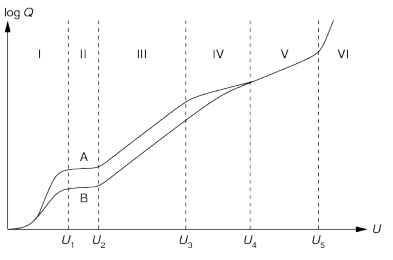
\includegraphics[width=\textwidth]{../Figures/total.PNG}
\caption{Total charge versus counter voltage.}
\label{fig:Total}
\end{figure}

\paragraph{Proportional Counter}

We have a cylindrical gas chamber, where in the middle of the chamber is the anode wire and the cylinder coat is the cathode.
We can create an electrical field $E$ proportional to $\frac{1}{r}$ so near the wire we get a high field.
If we put a high voltage (\SI{1}{kV}) through a resistance we get a gas amplification near the anode.

A proportional counter is good for energy measurement because of the probability between magnitude of voltage and energy of the particle.
We use it for detection of alpha and beta particles.

The characteristic curve is determined by puls rate in dependence of the applied voltage.

Only from a certain threshold voltage a certain puls height is reached so particle can be detected.

\begin{figure}[H]
\centering
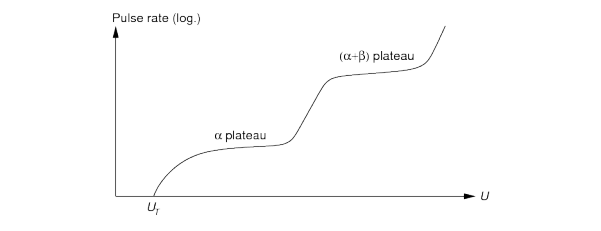
\includegraphics[width=\textwidth]{../Figures/prop.PNG}
\caption{Expected characteristic curve for proportional counter.}
\label{fig:Proportional}
\end{figure}


\paragraph{GM-counter}

The GM-counter is a proportional counter with a higher voltage that generates a much stronger electrical field.
This creates UV-photons, it comes to an avalanche along the whole anode wire.
At the same time we have to quench the gas after ionization, otherwise the ions of the cathode activate new electrons.



\begin{figure}[H]
\centering
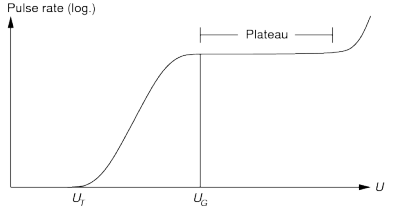
\includegraphics[width=\textwidth]{../Figures/Geiger.PNG}
\caption{Expected characteristic curve for Geiger counter.}
\label{fig:Geiger}
\end{figure}

From a certain threshold voltage the puls height is still dependent of the energy of the particle. After a certain Geiger threshold $U_G$ the pluses are the same heights for all particles.

\subsection{Statistics}

The first discrete distribution is the binomial distribution with the probability density:
$$ P(k) = \frac{{n!}}{{k!\left( {n - k} \right)!}}p^k (1-p)^{n - k} = \left( {\begin{array}{*{20}c} n \\ k \\ \end{array}} \right)p^k (1-p)^{n - k}$$
with the mean value of $\bar{k}=\mu=np$ and the standard deviation of $\sigma=\sqrt{np(1-p)}$

For large $n$ and small probability $p$ we obtain the Poisson distribution with $np= \mu=const$:
$$P\left( k \right) = \frac{{e^{ - \mu } \mu ^k }}{{k!}}$$
with $\bar{k}=\mu$ and $\sigma=\sqrt{\mu}$.

From this for large $\mu$ ($\mu>10$) we get the normal distribution:
$$P(k) = \frac{1}{{\sigma \sqrt {2\pi } }}e^{{{ - \left( {k - \mu } \right)^2 } \mathord{\left/ {\vphantom {{ - \left( {k - \mu } \right)^2 } {2\sigma ^2 }}} \right. \kern-\nulldelimiterspace} {2\sigma ^2 }}}$$
if $\mu$ and $\sigma$ are not independent, we get the relation $\sigma =\sqrt{\mu}$.

Finally, there is the exponential distribution:
\begin{equation}\label{eq:exp}
	\rho(\Delta t)= A\exp(-A\Delta t)
\end{equation}


Furthermore, one considers the $\chi^2$ distribution as a measurement of the goodness of a fit to the measured values:
$$\chi^2(a)=\sum_{i=1}^{n}{\dfrac{(x_i-y_i(a))^2}{\sigma_i^2}}.$$
For a good fit, the value should be in the range of degrees of freedom.
By minimizing the $\chi^2$ one gets the parameters.
The value for the integrated $\chi^2$ distribution from zero to infinity gives the probability for re-measurement of a higher value for the $\chi^2$.
It should therefore be very high, so one can say that the minimal $\chi^2$ was found.

\section{Measurments with the Geiger counter}

\subsection{Setup} \label{sec:GM}

As radioactive source we will use ${}^{90}$Sr. The activity of the source on the day of the experiment is shown in \cref{tab:Activity}, together with the sources needed for the proportional counter. When used, the probe is placed inside a sealed lead chamber with the Geiger-Mueller-counter. The signal goes through a multiplier before it is goes into the electronic counter. We also have an oscilloscope, a dead time stage and a 1-MHz-generator we can introduce to the circuit when needed.

\begin{table}[H]
        \renewcommand{\arraystretch}{1}
        \centering
        \Large
        \begin{adjustbox}{width=\textwidth}
                \begin{tabular}{|c|c|c|c|}
                        \hline
                        & ${}^{241}$Am & ${}^{90}$Sr & ${}^{14}$C \\
                        \hline
                        Buy date & 07.03.1986 & 04.01.1974 & 03.10.2004 \\
                        \hline
                        Activity at buy date (kBq) & $3570$ & $185$ & $1$ \\
                        \hline
                        Halflife time (years) & $\left(4.326 \pm 0.006\right) \times 10^{2}$ & $\left(2.890 \pm 0.003\right) \times 10^{1}$ & $\left(5.70 \pm 0.03\right) \times 10^{3}$ \\
                        \hline
                        Decay constant (1/s) & $\left(5.209 \pm 0.007\right) \times 10^{-11}$ & $\left(7.798 \pm 0.008\right) \times 10^{-10}$ & $\left(3.95 \pm 0.02\right) \times 10^{-12}$ \\
                        \hline
                        Activity today (kBq) & $\left(3.3814 \pm 0.0003\right) \times 10^{3}$ & $\left(6.085 \pm 0.007\right) \times 10^{1}$ & $\left(9.98200 \pm 0.00009\right) \times 10^{-1}$ \\
                        \hline
                \end{tabular}
        \end{adjustbox}
        \caption{Activities of sources on the day of the experiment.}
        \label{tab:Activity}
\end{table}   

\subsection{Procedure}

First we placed a ${}^{90}$Sr-Probe in a lead chamber and measured the count rate's dependence on the voltage.

Next we checked the intensity of the background, by measuring the pulse rate without a probe in the chamber and found it to be $\frac{4}{\SI{10}{s}}$.

Then, using the oscilloscope we produced a Stever diagram to estimate the dead time and the recover time.

Since we will need to use the dead time stage to find the resolution time of the counter, we first need to verify the electronically generated dead times indicated on it. We do this by connenting it to a 1-MHz-generator and writing down the count rates for each dead time.

Now we can make the pulses from the Geiger counter pass through the dead time stage. We measure the pulse rate for the large and the small dead time, writing down three pulse rate for each.

\subsection{Analysis}

For the error calculation in this and all further analysis we will use Gaussian error propagation. In complicated cases we use the Python package \code{uncertainties}, which implements numerical calculations of error propagation using automatic differentiation methods, to compute the errors.

\subsubsection{Characterization of dead time}

First of all we generated a pulse of $1\,MHz$ with the generator
that is linked to the variable dead time stage (with settings $2\, ms$ and $1\mu s$) and wrote down the count (counts over $2\, s$ measured $3$ times).
With
\begin{equation}
N =\frac{n_1}{1-n_1\cdot\tau_1}=\frac{n_2}{1-n_2\cdot\tau}
\end{equation}
we can correct the stage if we consider that the smaller stage is correct 
with a measured count rate of $10^6$ for $1\mu s$ and 
$519.67\pm0.07$ for $2\,ms$ we get a corrected dead time of $1.92\,ms$.

Now we can calculate with the same method the resolution time of the GM-counter.
We assume that the real dead time is between $\SI{1}{\micro s}$ and $\SI{2}{ms}$. With the formula
\begin{equation}
\tau =\frac{1}{n_2}-\frac{1}{n_1}+\tau_1
\end{equation}
and $n_2=\SI{179.6\pm0.6}{s^{-1}}$, $n_1=\SI{246.0\pm1.8}{s^{-1}}$ we got a resolution time of $\tau=\SI{422\pm35}{ms}$.

\subsubsection{Stever diagram}

With a Stever diagram we can estimate the resolution time on the oscilloscope out of the dead time an the recovery time that we can read from the scope. 

The dead time is the distance between the main peak and the next incoming peak, during that time the GM-Counter can not detect anything.
We estimate the dead time with $\SI{224 \pm 4}{\micro s}$ (for that we read the dead time out of the steverdiagram 3 time with a min and max value and mean over all)
The recovery time is the distance bewteen main peak and the next main peak, we estimated it as $\SI{505\pm11}{\micro s}$ (same method as before).

\begin{figure}[H]
	\centering
	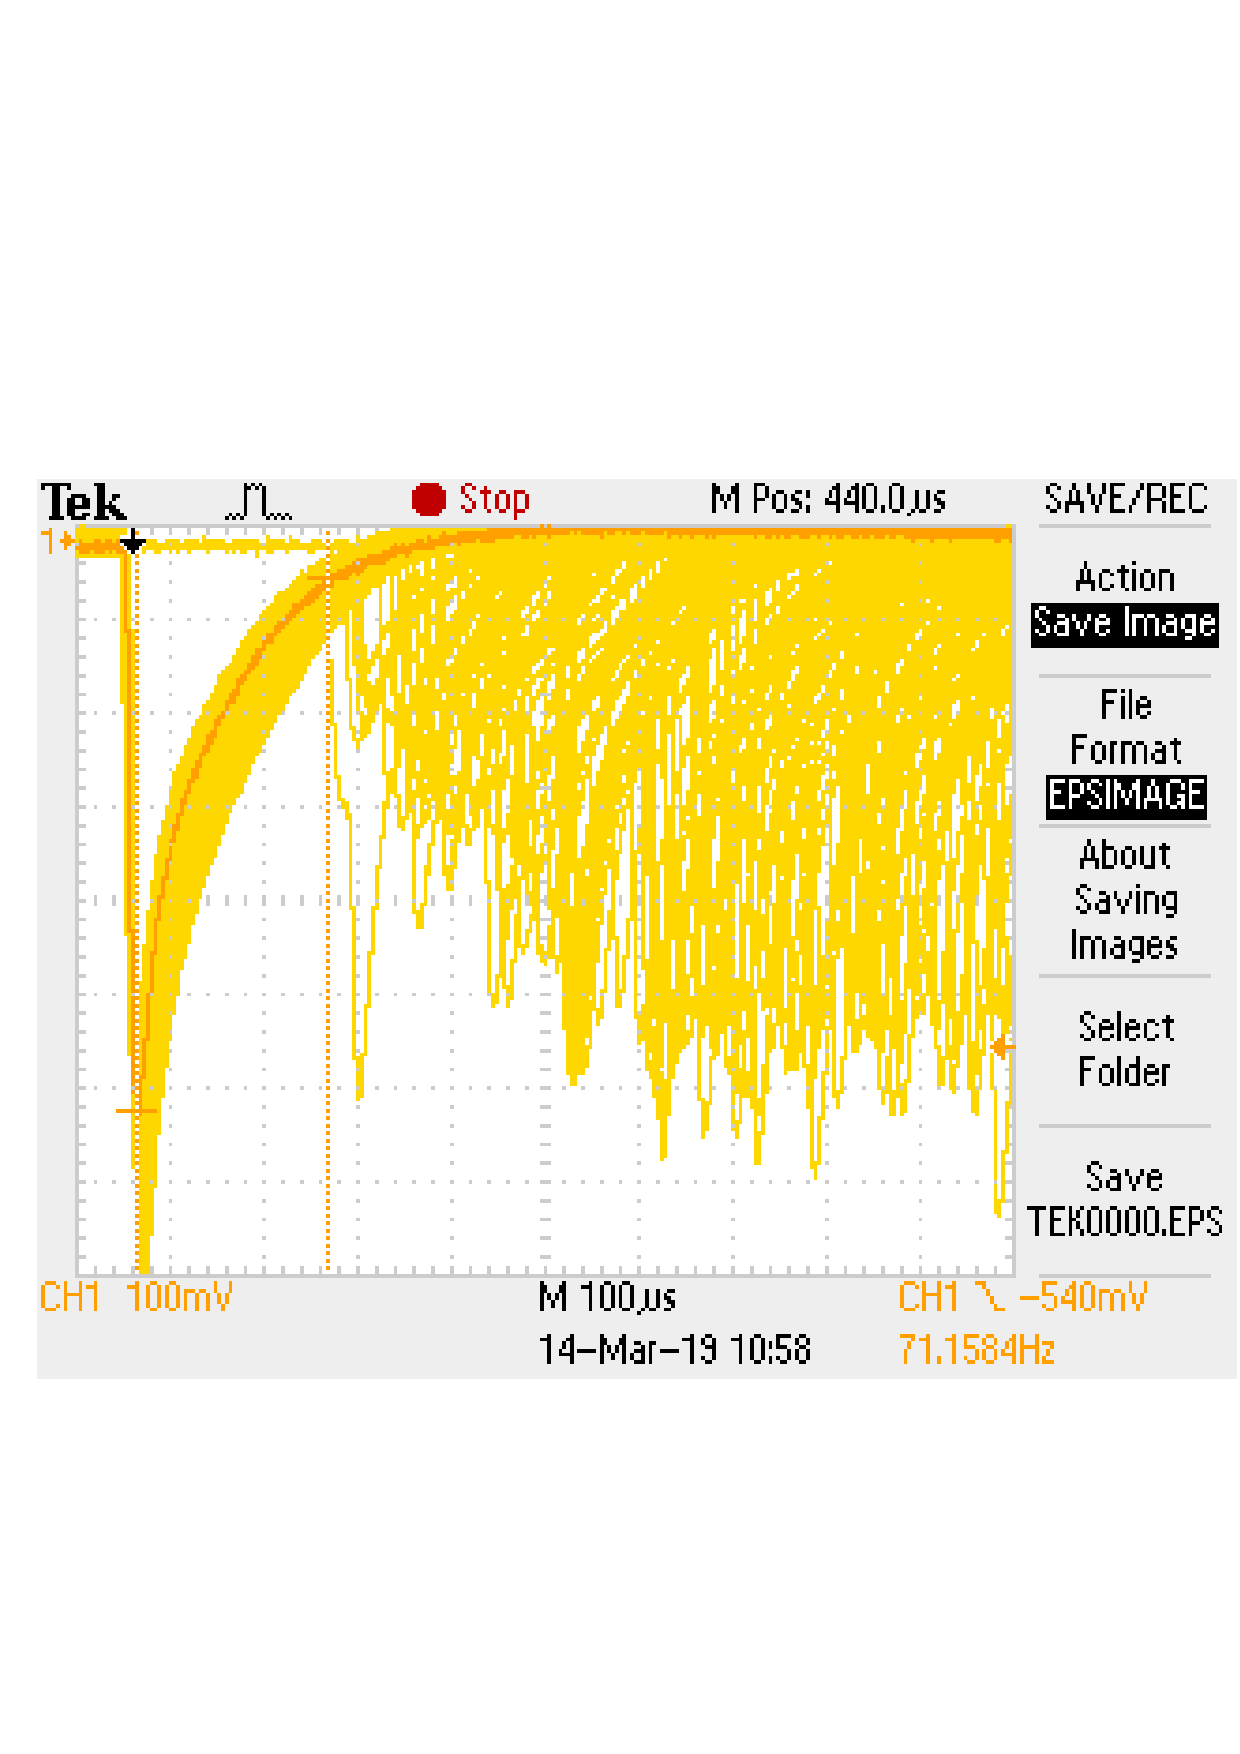
\includegraphics[width=\textwidth]{../Figures/TEK0000.pdf}
	\caption{Stever diagram with markers set to measure dead time.}
	\label{fig:SteverDead}
\end{figure}

\begin{figure}[H]
	\centering
	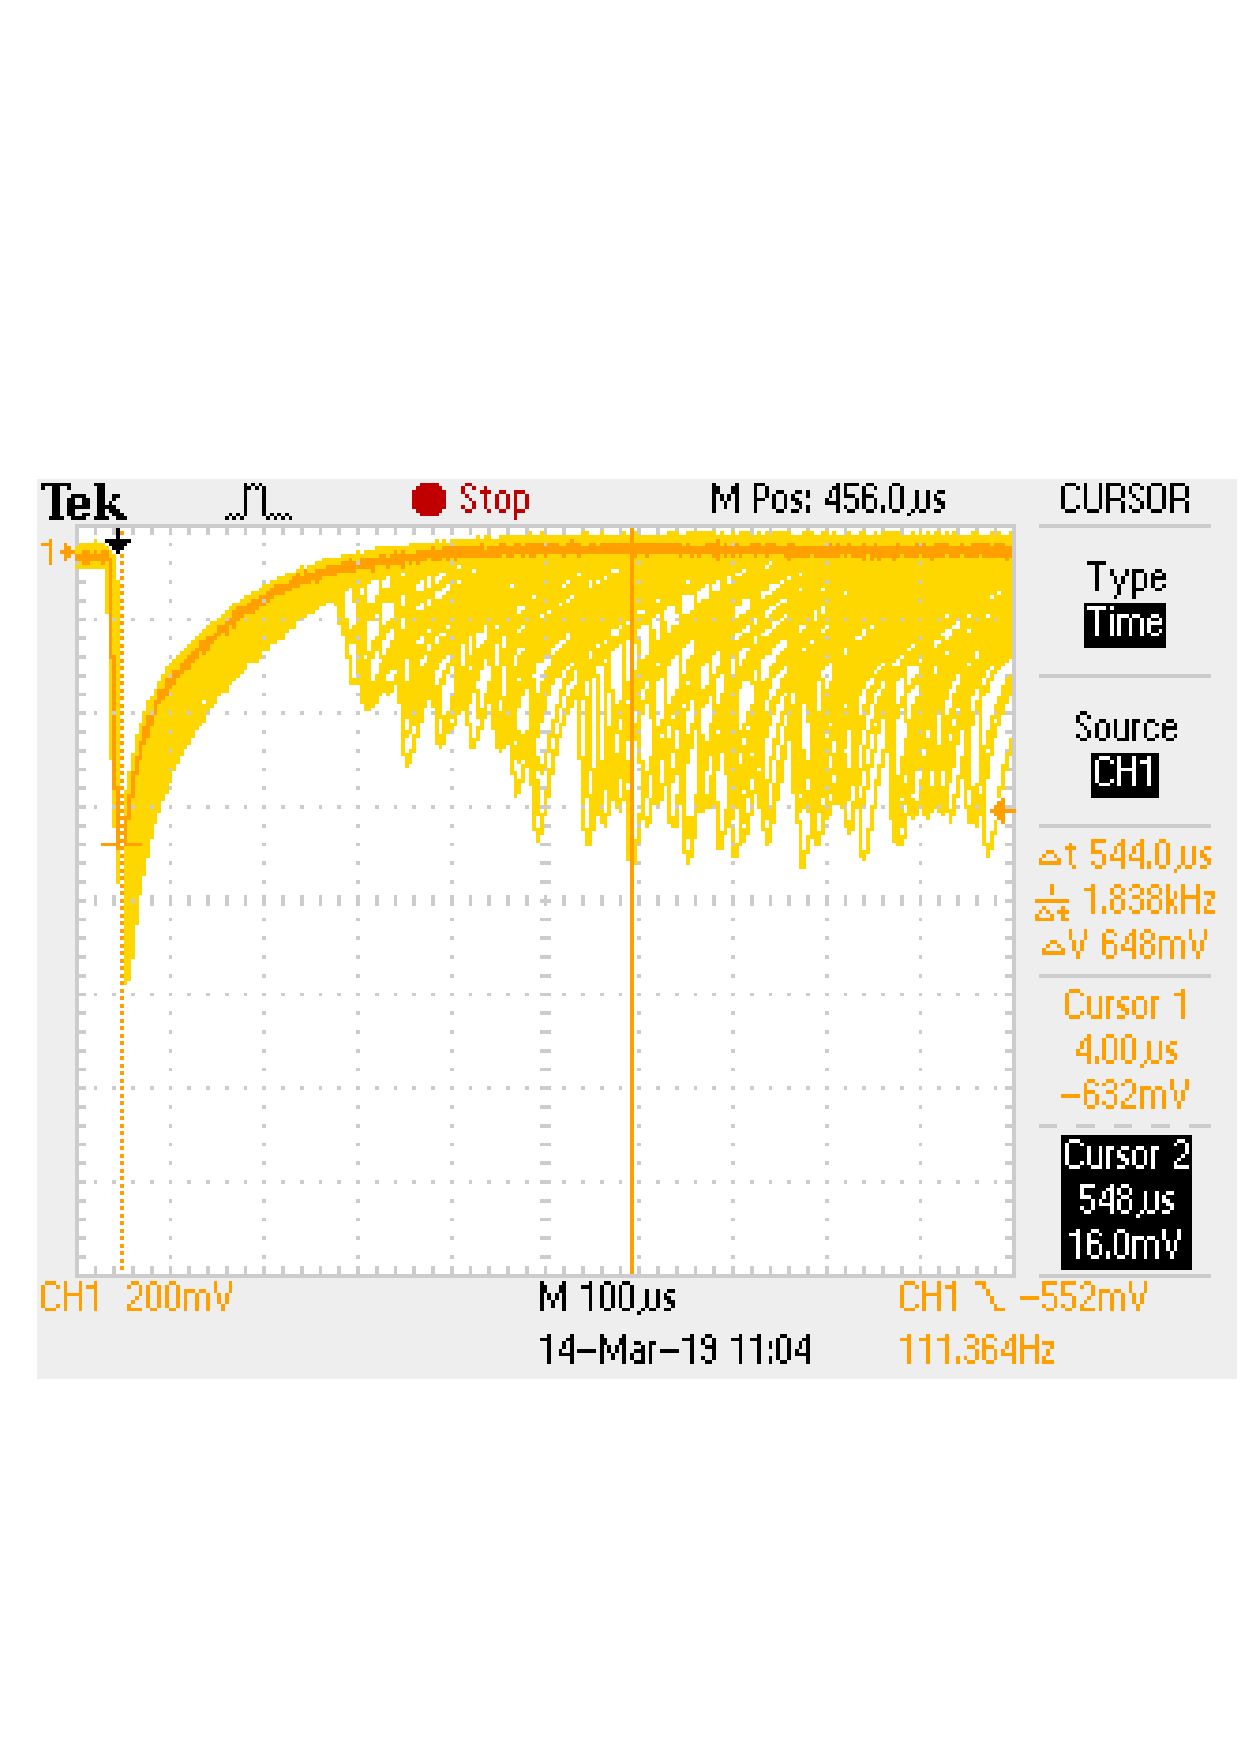
\includegraphics[width=\textwidth]{../Figures/F0001TEK.pdf}
	\caption{Stever diagram with markers set to measure recovery time.}
	\label{fig:SteverRecovery}
\end{figure}

\subsubsection{Characteristic curve of GM-Counter}
After the dead time correction we can now study the characteristic Geiger curve.
We plot the voltage (in 10 Volt steps) over the measured counts per 1s ($\frac{\mathrm{actual\,counts}}{10\,s}$).

With the calculated resolution time we can now correct the characteistic GM-curve for the detected counts with $N =\frac{n}{1-n\cdot\tau}$. 
For errors we used the uncertainties package for python, which calculates errors with gaussian propagation.

\begin{figure}[H]
\centering
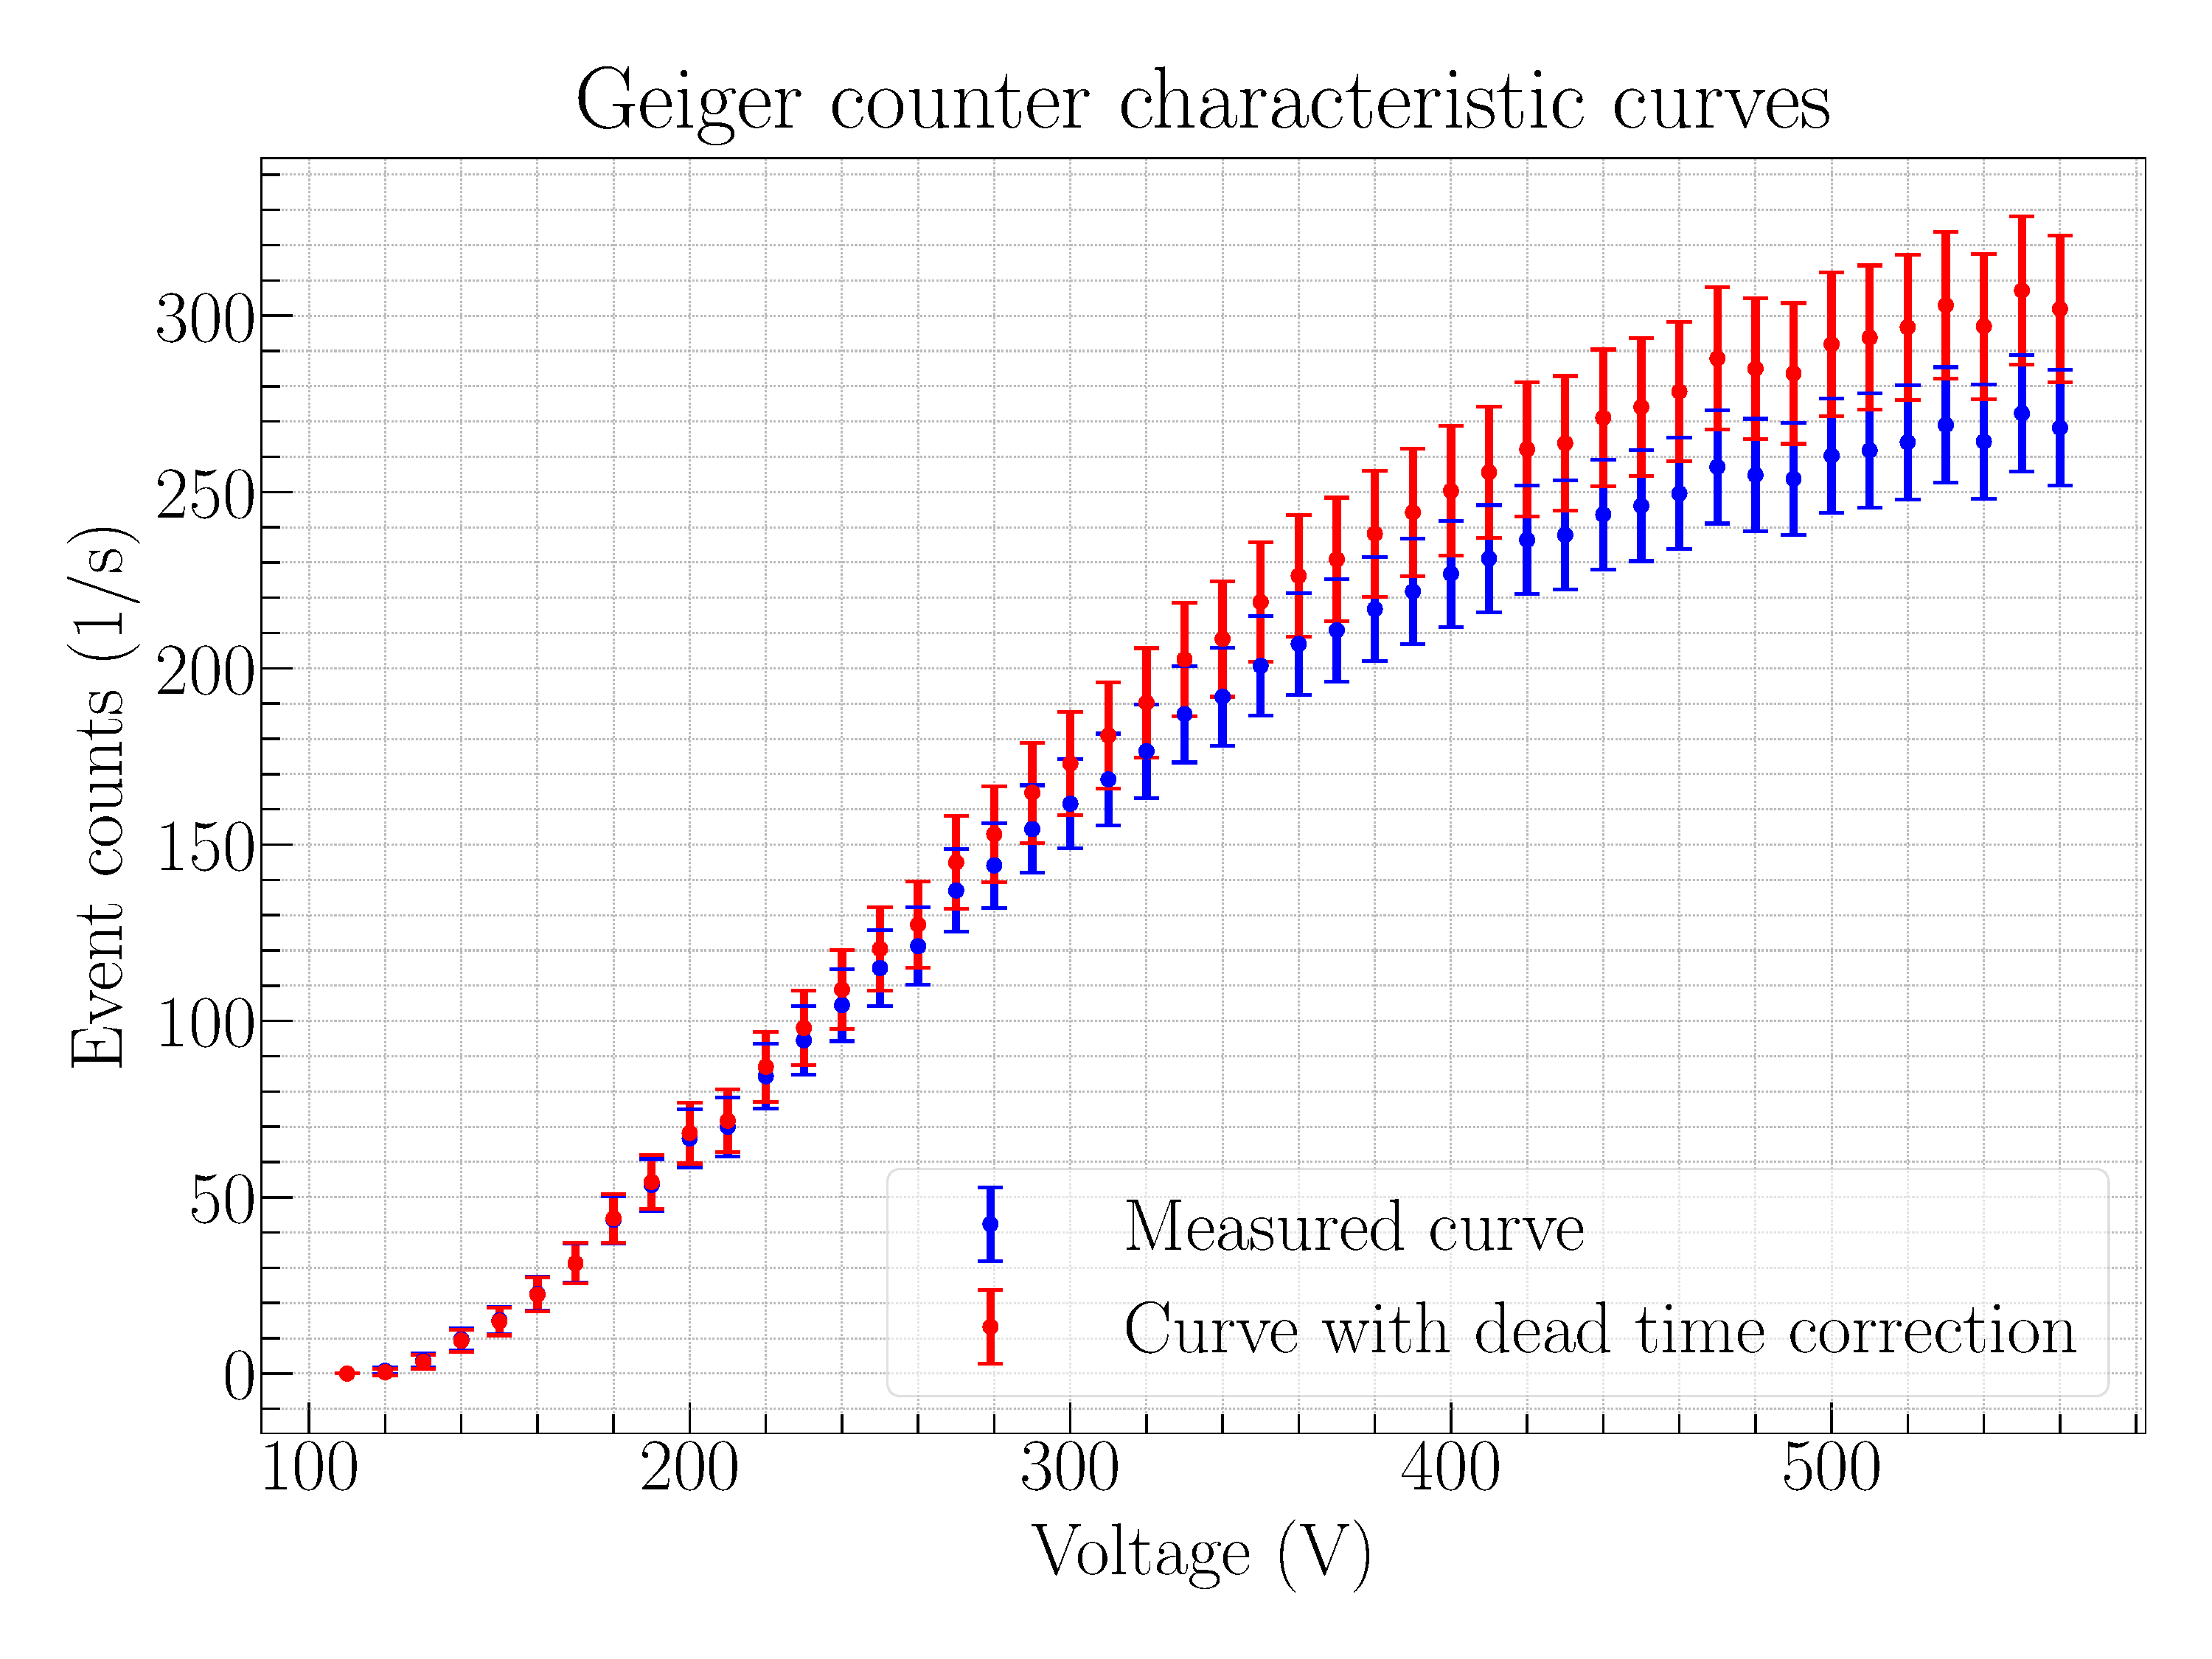
\includegraphics[width=\textwidth]{../Figures/Geiger_characteristic_curves.pdf}
\caption{GM-counter characteristic curves with deadtime correction}
\label{fig:GeigerCorect}
\end{figure}

\section{Measurement of statistical distributions}

\subsection{Setup}

We are still using the setup of the Geiger counter for this part, which was described in \cref{sec:GM}. 

\subsection{Procedure}

First we set the measurement, such that an average of at least 25 events were recorded per measurement, while the Sr-probe was in the detector. We found $10\,s$ to be a good interval. Then we measured the number of events per $10\,s$, 100 times.

Next we removed the probe from the chamber and set the measurement time, such that the average event count per measurement was at most 2. There we found $2\,s$ to be a good intervall. Then we measured the number of events per $2\,s$, 113 times.

Next we placed the probe in the chamber again and used the oscilloscope to take a shot of the pulses on a $50\,ms$ scale. We will use this data to measure the times between two consecutive events.

We repeated the last measurement with an alternative method: using the counter we recorded the counts per $0.1\,s$ 50 times.

\subsection{Analysis}

\subsubsection{Gaussian distribution}

In \cref{fig:GaussHist} we see the recorded count rates for the Geiger counter with the Sr-probe in a histogramm, that vaguely resemble a gaussian distribution. We calculated the mean and standard deviation of our data and with those calculated our expected gauss distribution, according to
\begin{equation}
P(k) = \frac{1}{\sqrt{2\pi}\sigma} \exp(-\frac{(k-\mu)^2}{2\sigma^2}).
\end{equation}
This expected curve is shown in \cref{fig:GaussFit} together with the normalized histogramm of the count rates. In the same figure we also plotted a gauss curve we fitted with the least square method with $\mu$ and $\sigma$ as free parameters. The mean values (including the error on mean) and standard deviations for both curves can be seen in \cref{tab:DistPara}.

\begin{figure}[H]
\centering
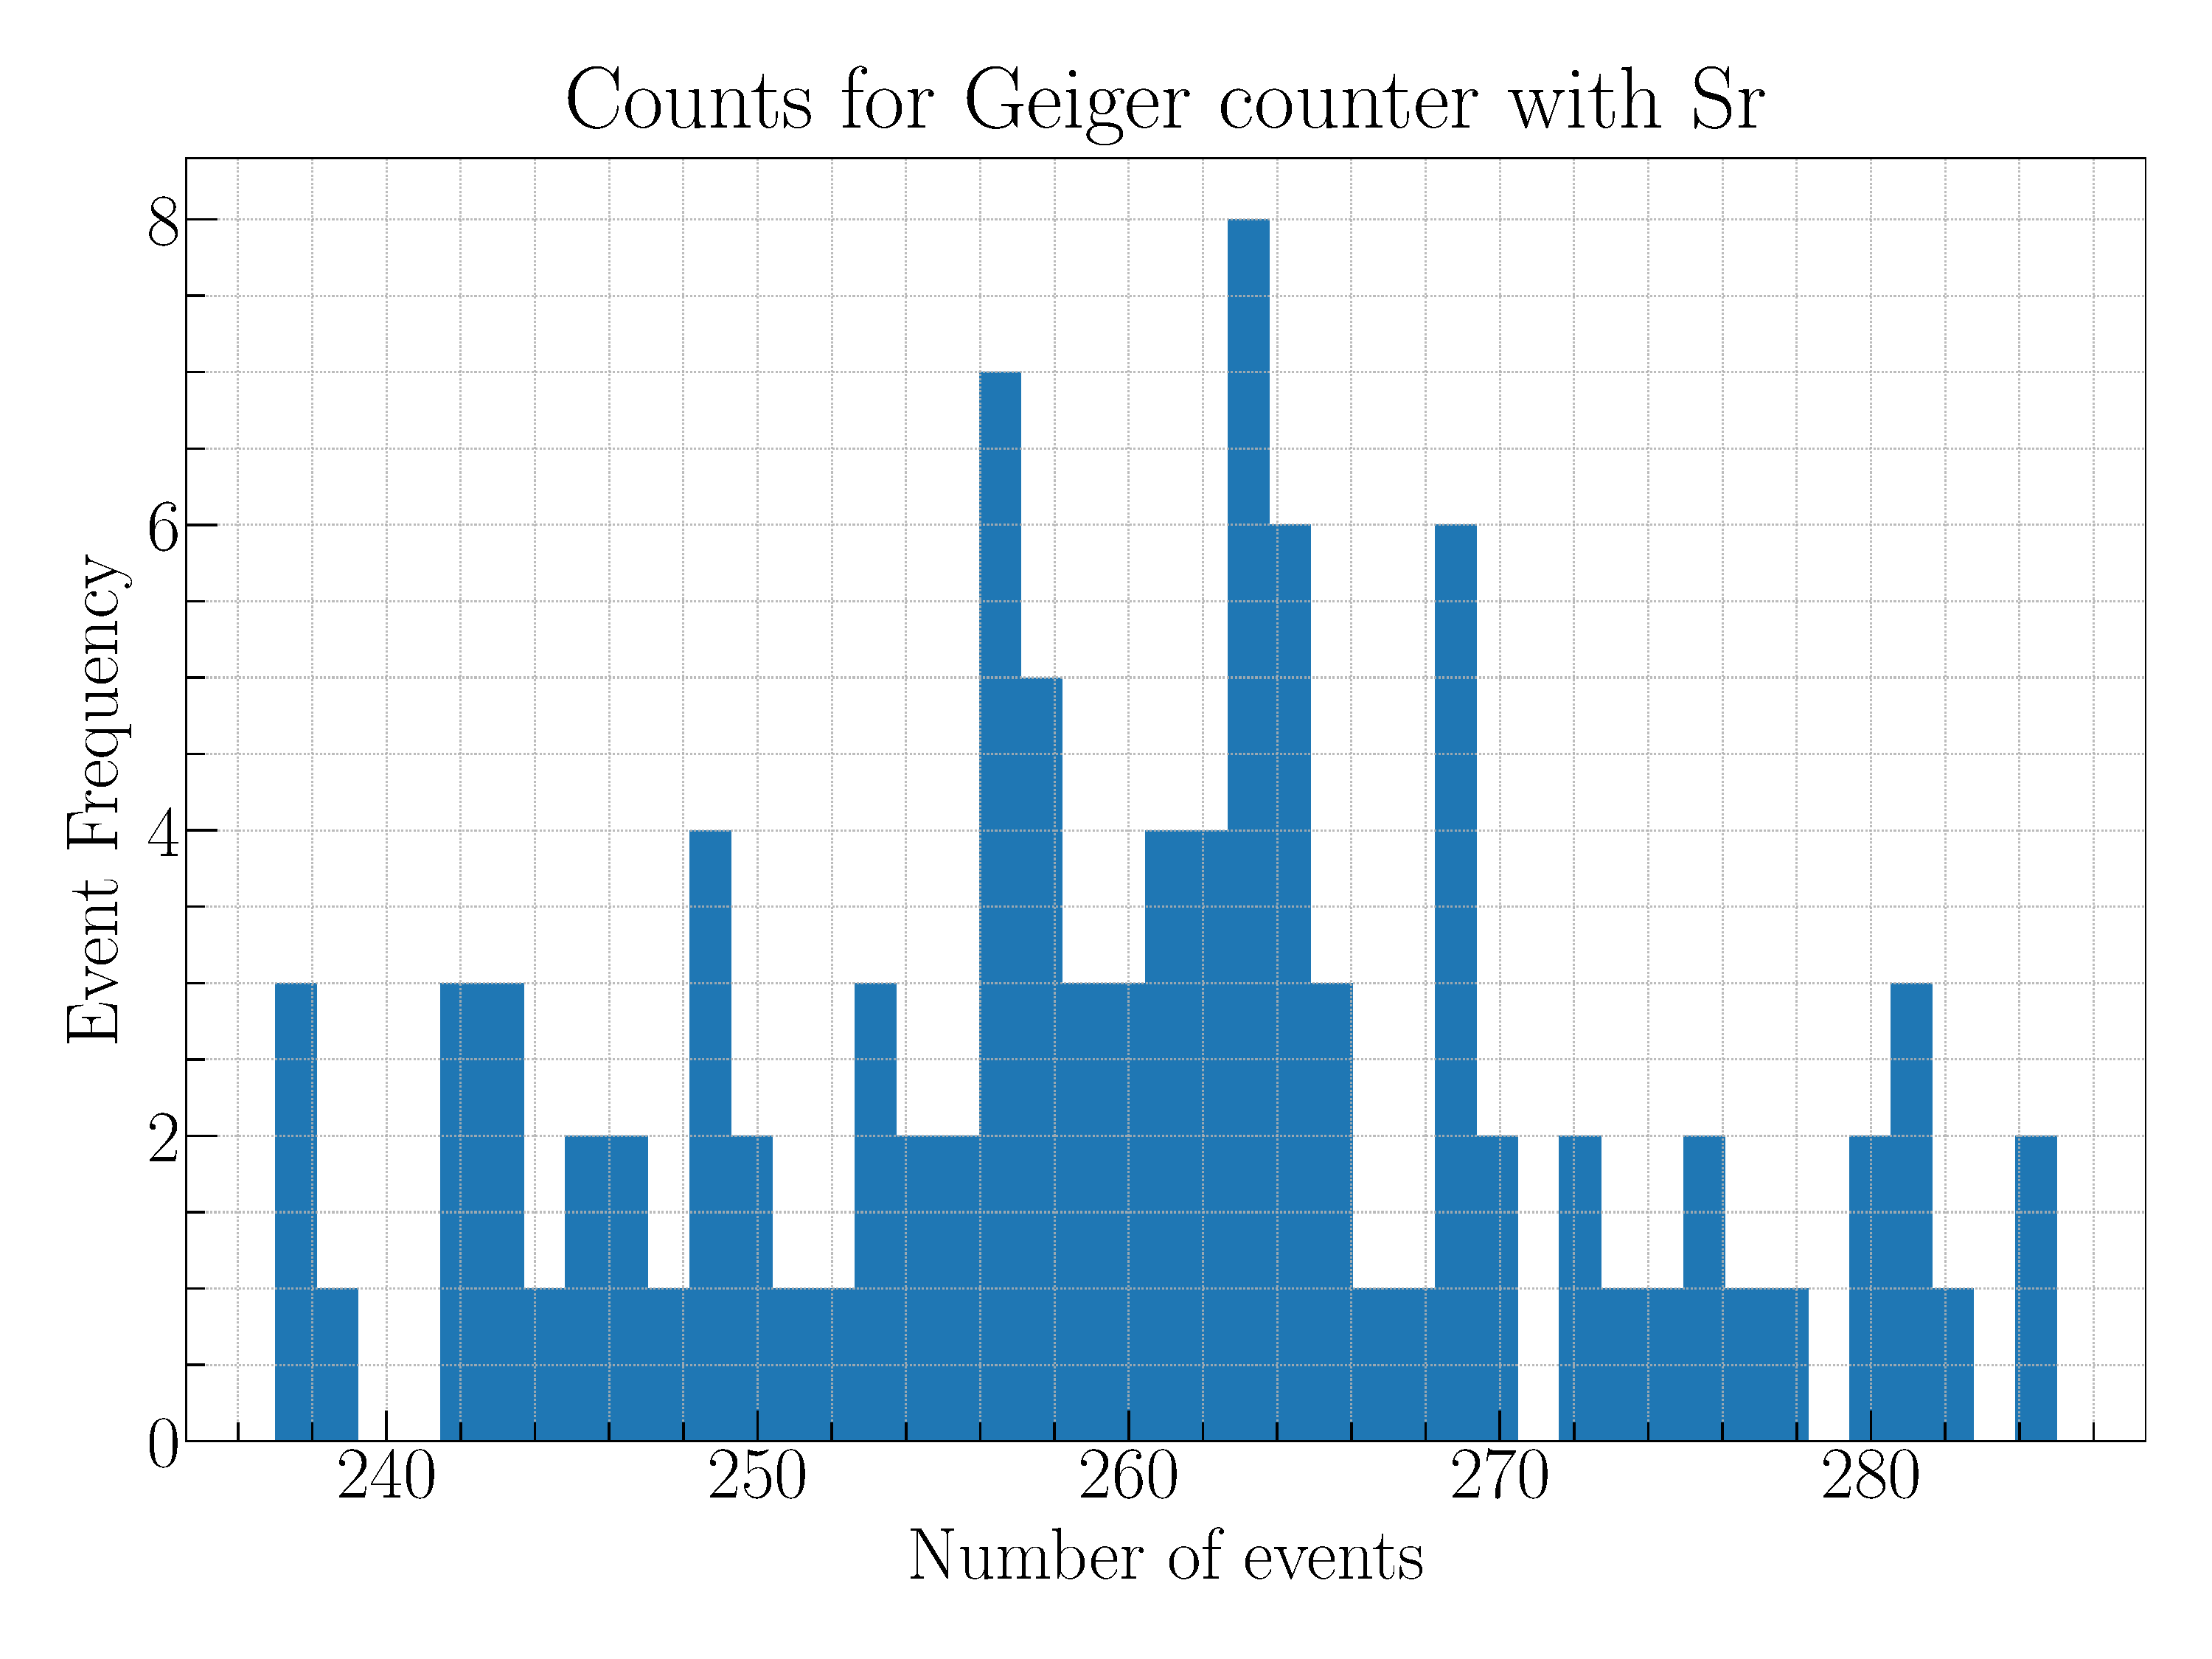
\includegraphics[width=0.9\textwidth]{../Figures/Geiger_gauss_histogram.pdf}
\caption{Pulse rate histogram with Sr.}
\label{fig:GaussHist}
\end{figure}

\begin{figure}[H]
\centering
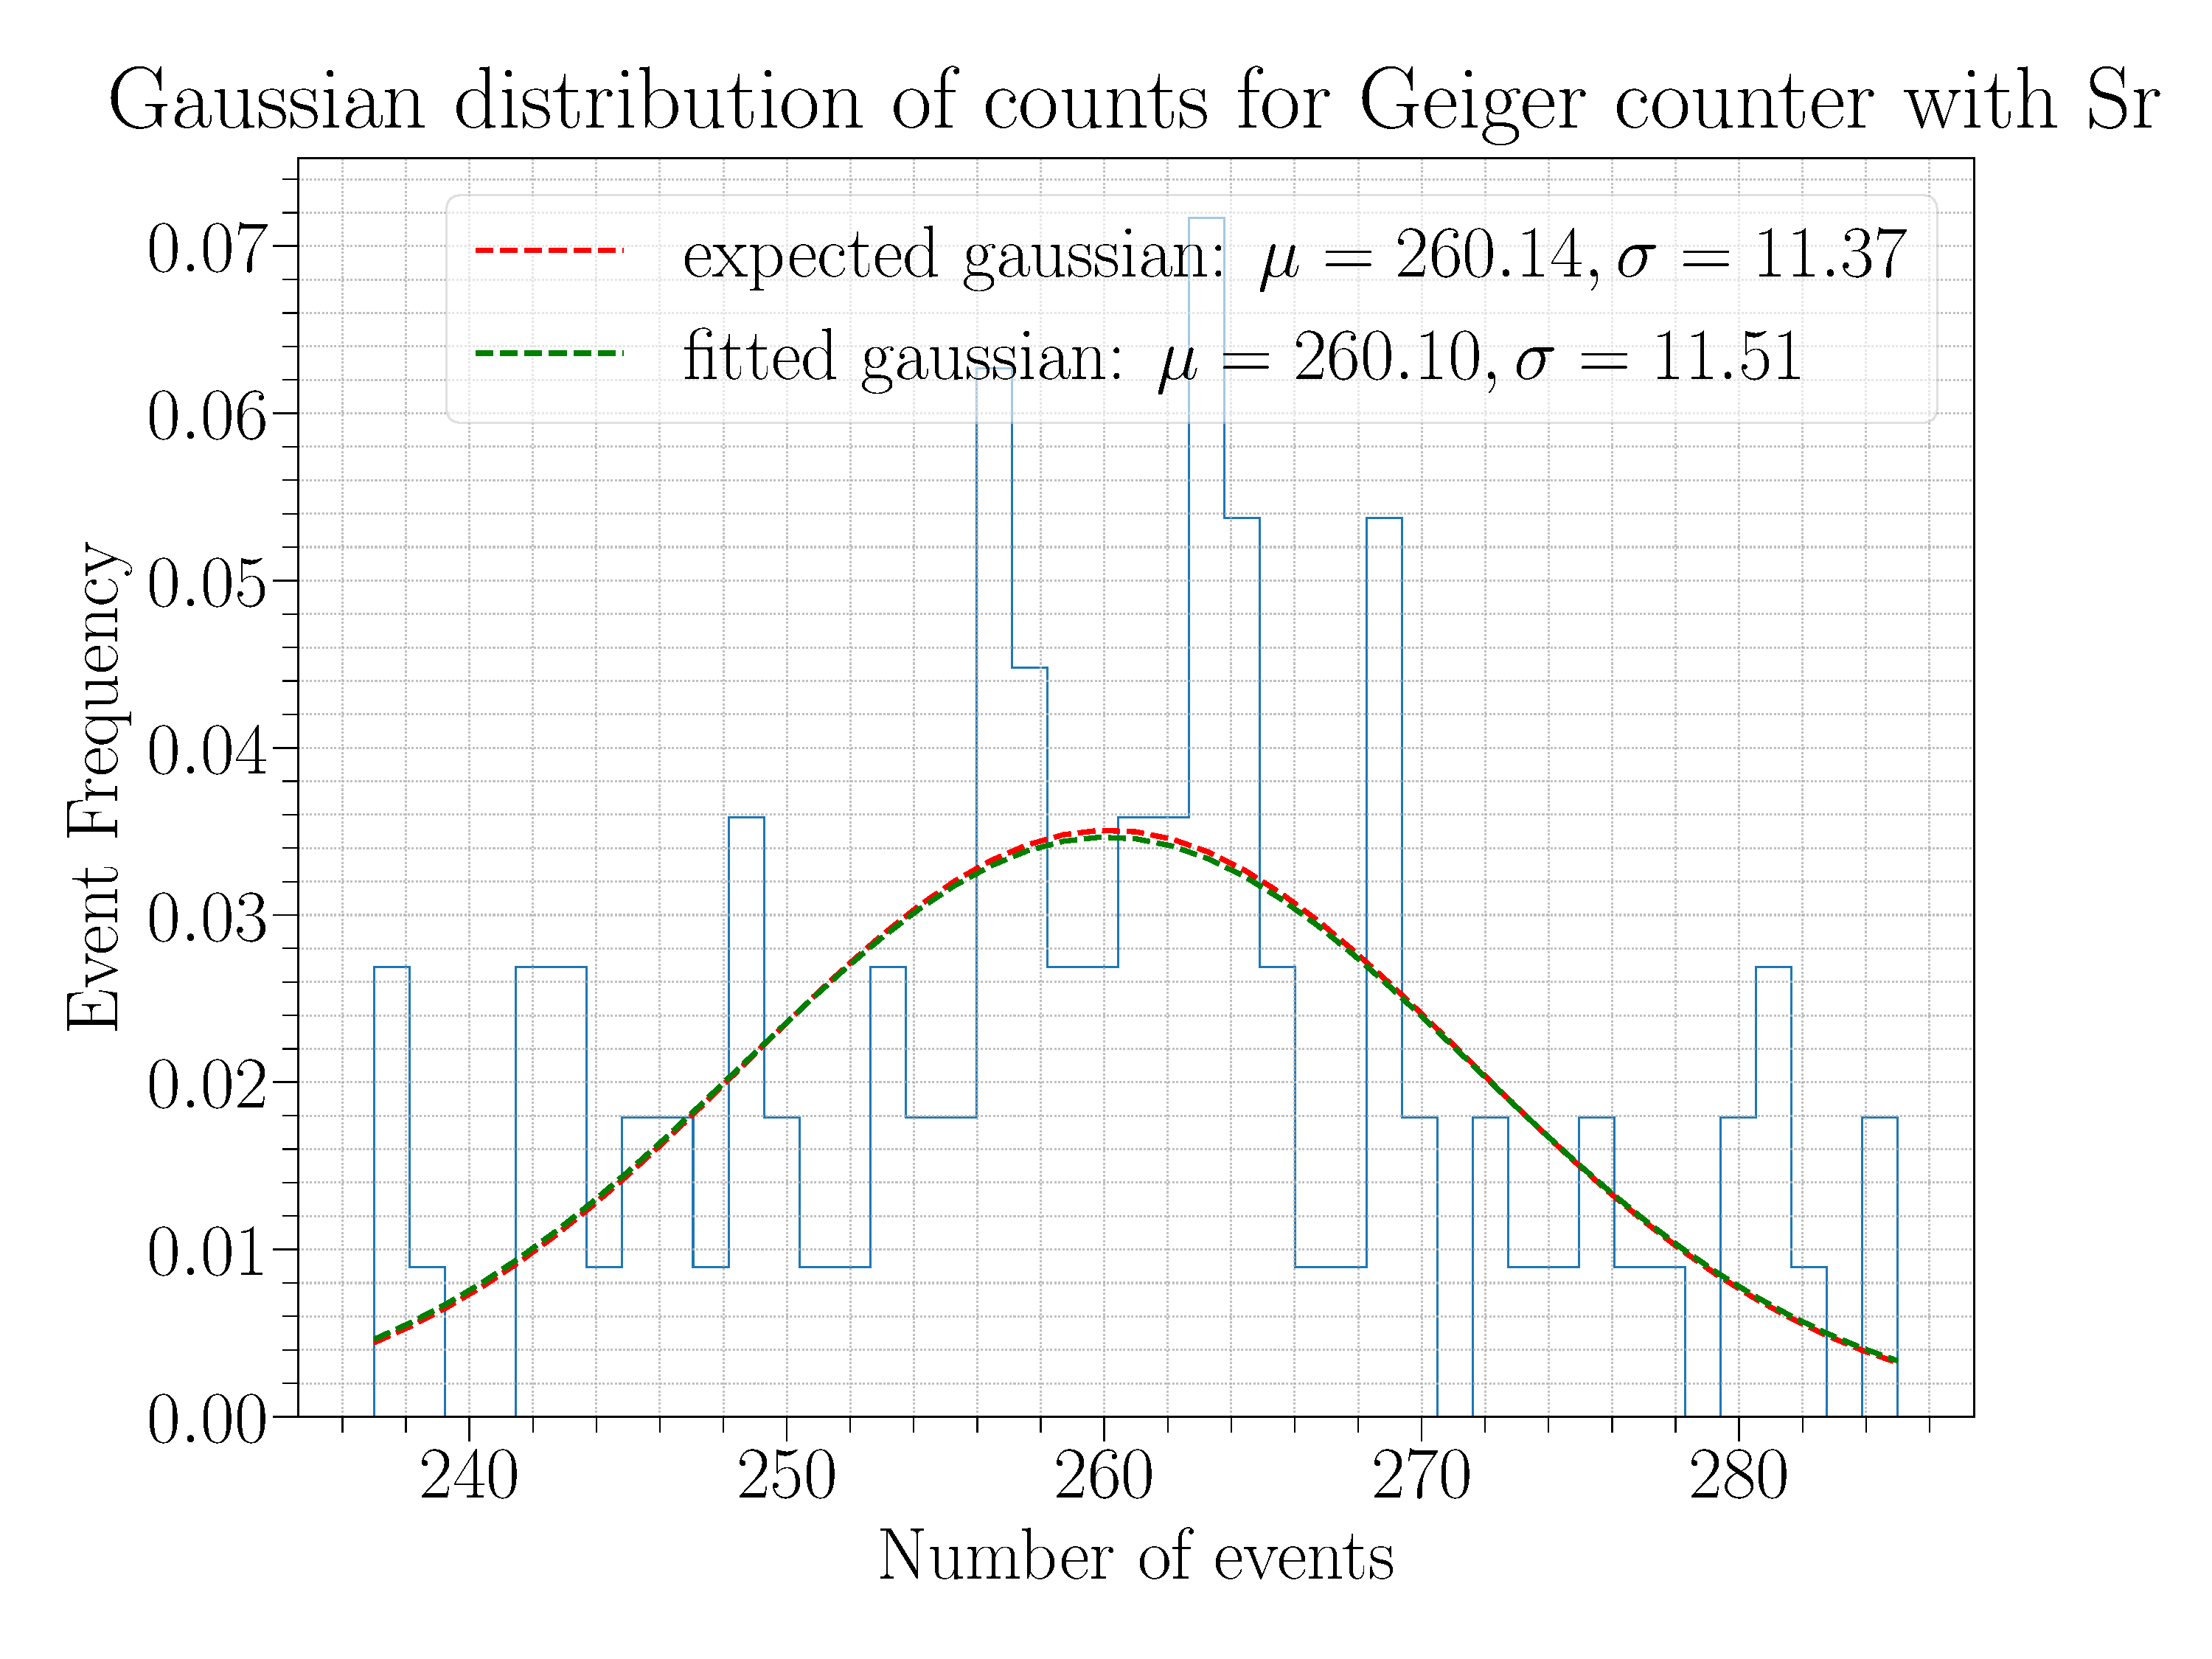
\includegraphics[width=0.9\textwidth]{../Figures/Geiger_gauss_fit.pdf}
\caption{Normalized histogram with expected and fitted gauss curves.}
\label{fig:GaussFit}
\end{figure}

\subsubsection{Poisson distribution}

We proceed analogously for the count rates of the empty Geiger counter. In \cref{fig:PoissonHist} we see the measured count rates and in \cref{fig:PoissonFit} we plotted the normalized histogramm, together with both the expected and the fitted poisson distribution
\begin{equation}
P(k) = \frac{\mu^k e^{-\mu}}{k!}.
\end{equation}
Of course here we only have one parameter, the mean value $\mu$, since the standard deviation is given by $\sigma = \sqrt{\mu}$. The mean values (including the error on mean) and standard deviations for both curves can be seen in \cref{tab:DistPara}. The errors on the standard deviations are come from the errors on the mean values through gaussian propagation.

\begin{figure}[H]
\centering
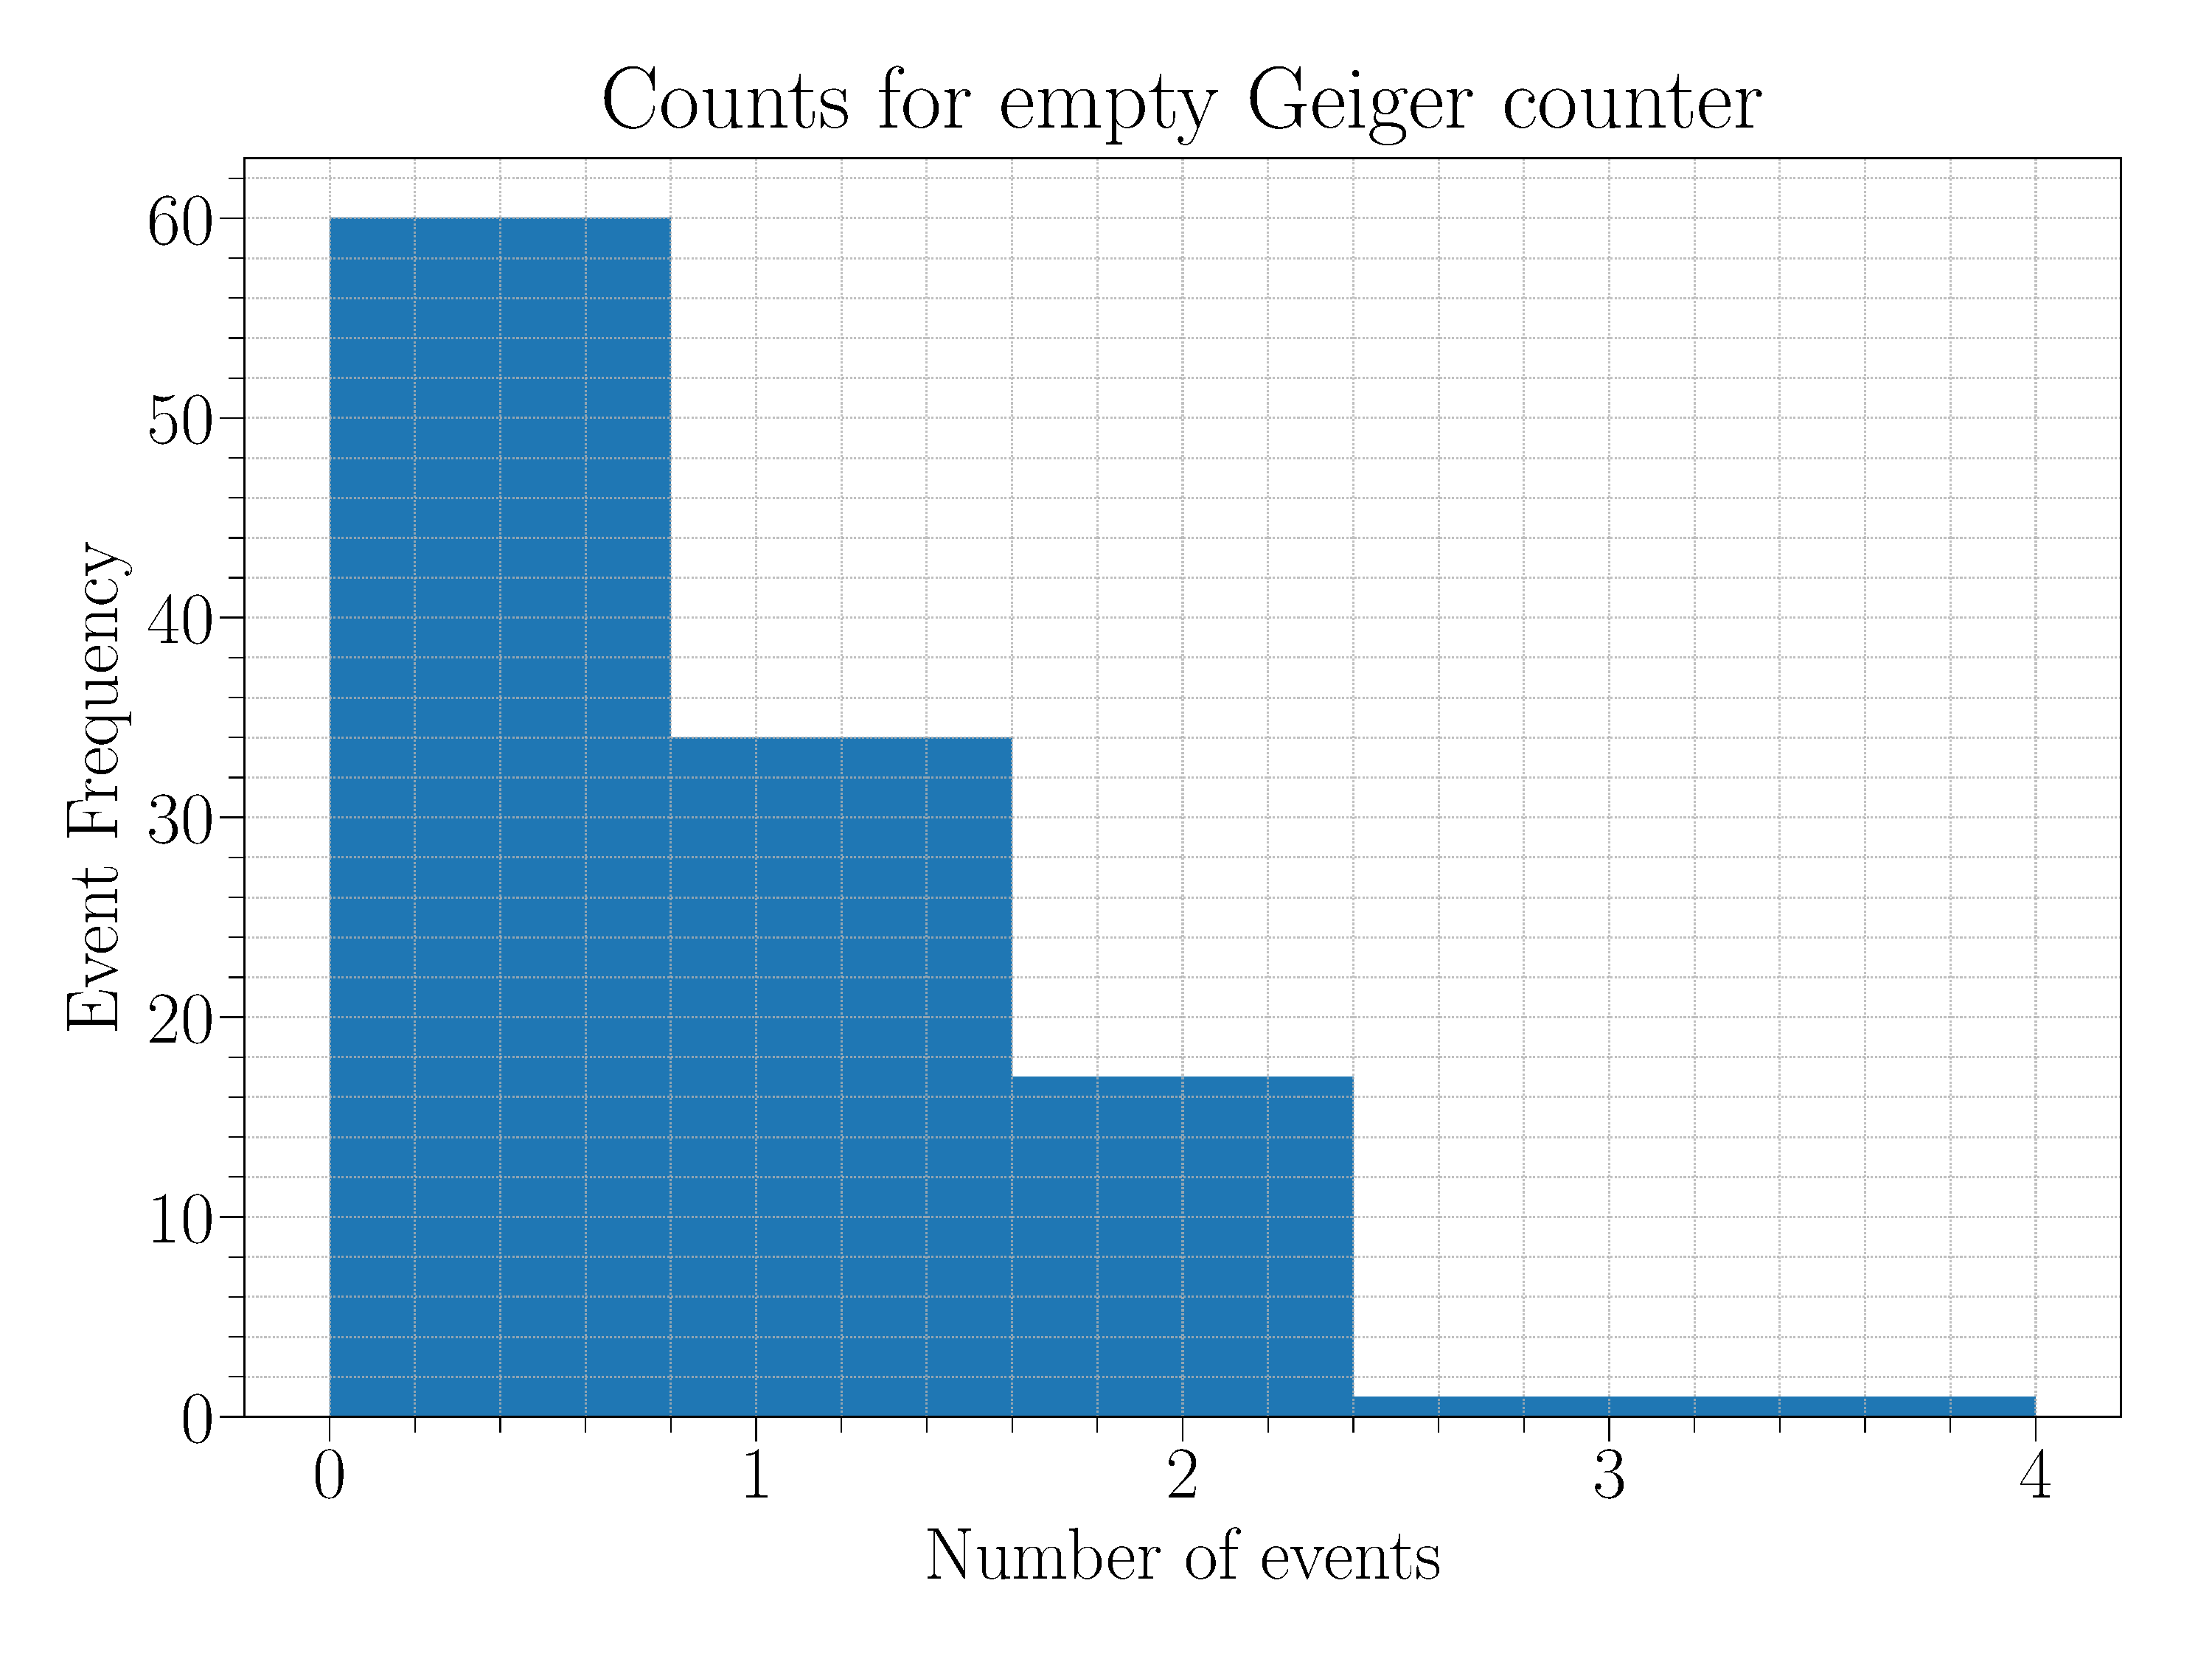
\includegraphics[width=0.9\textwidth]{../Figures/Geiger_poisson_histogram.pdf}
\caption{Pulse rate histogram for empty counter.}
\label{fig:PoissonHist}
\end{figure}

\begin{figure}[H]
\centering
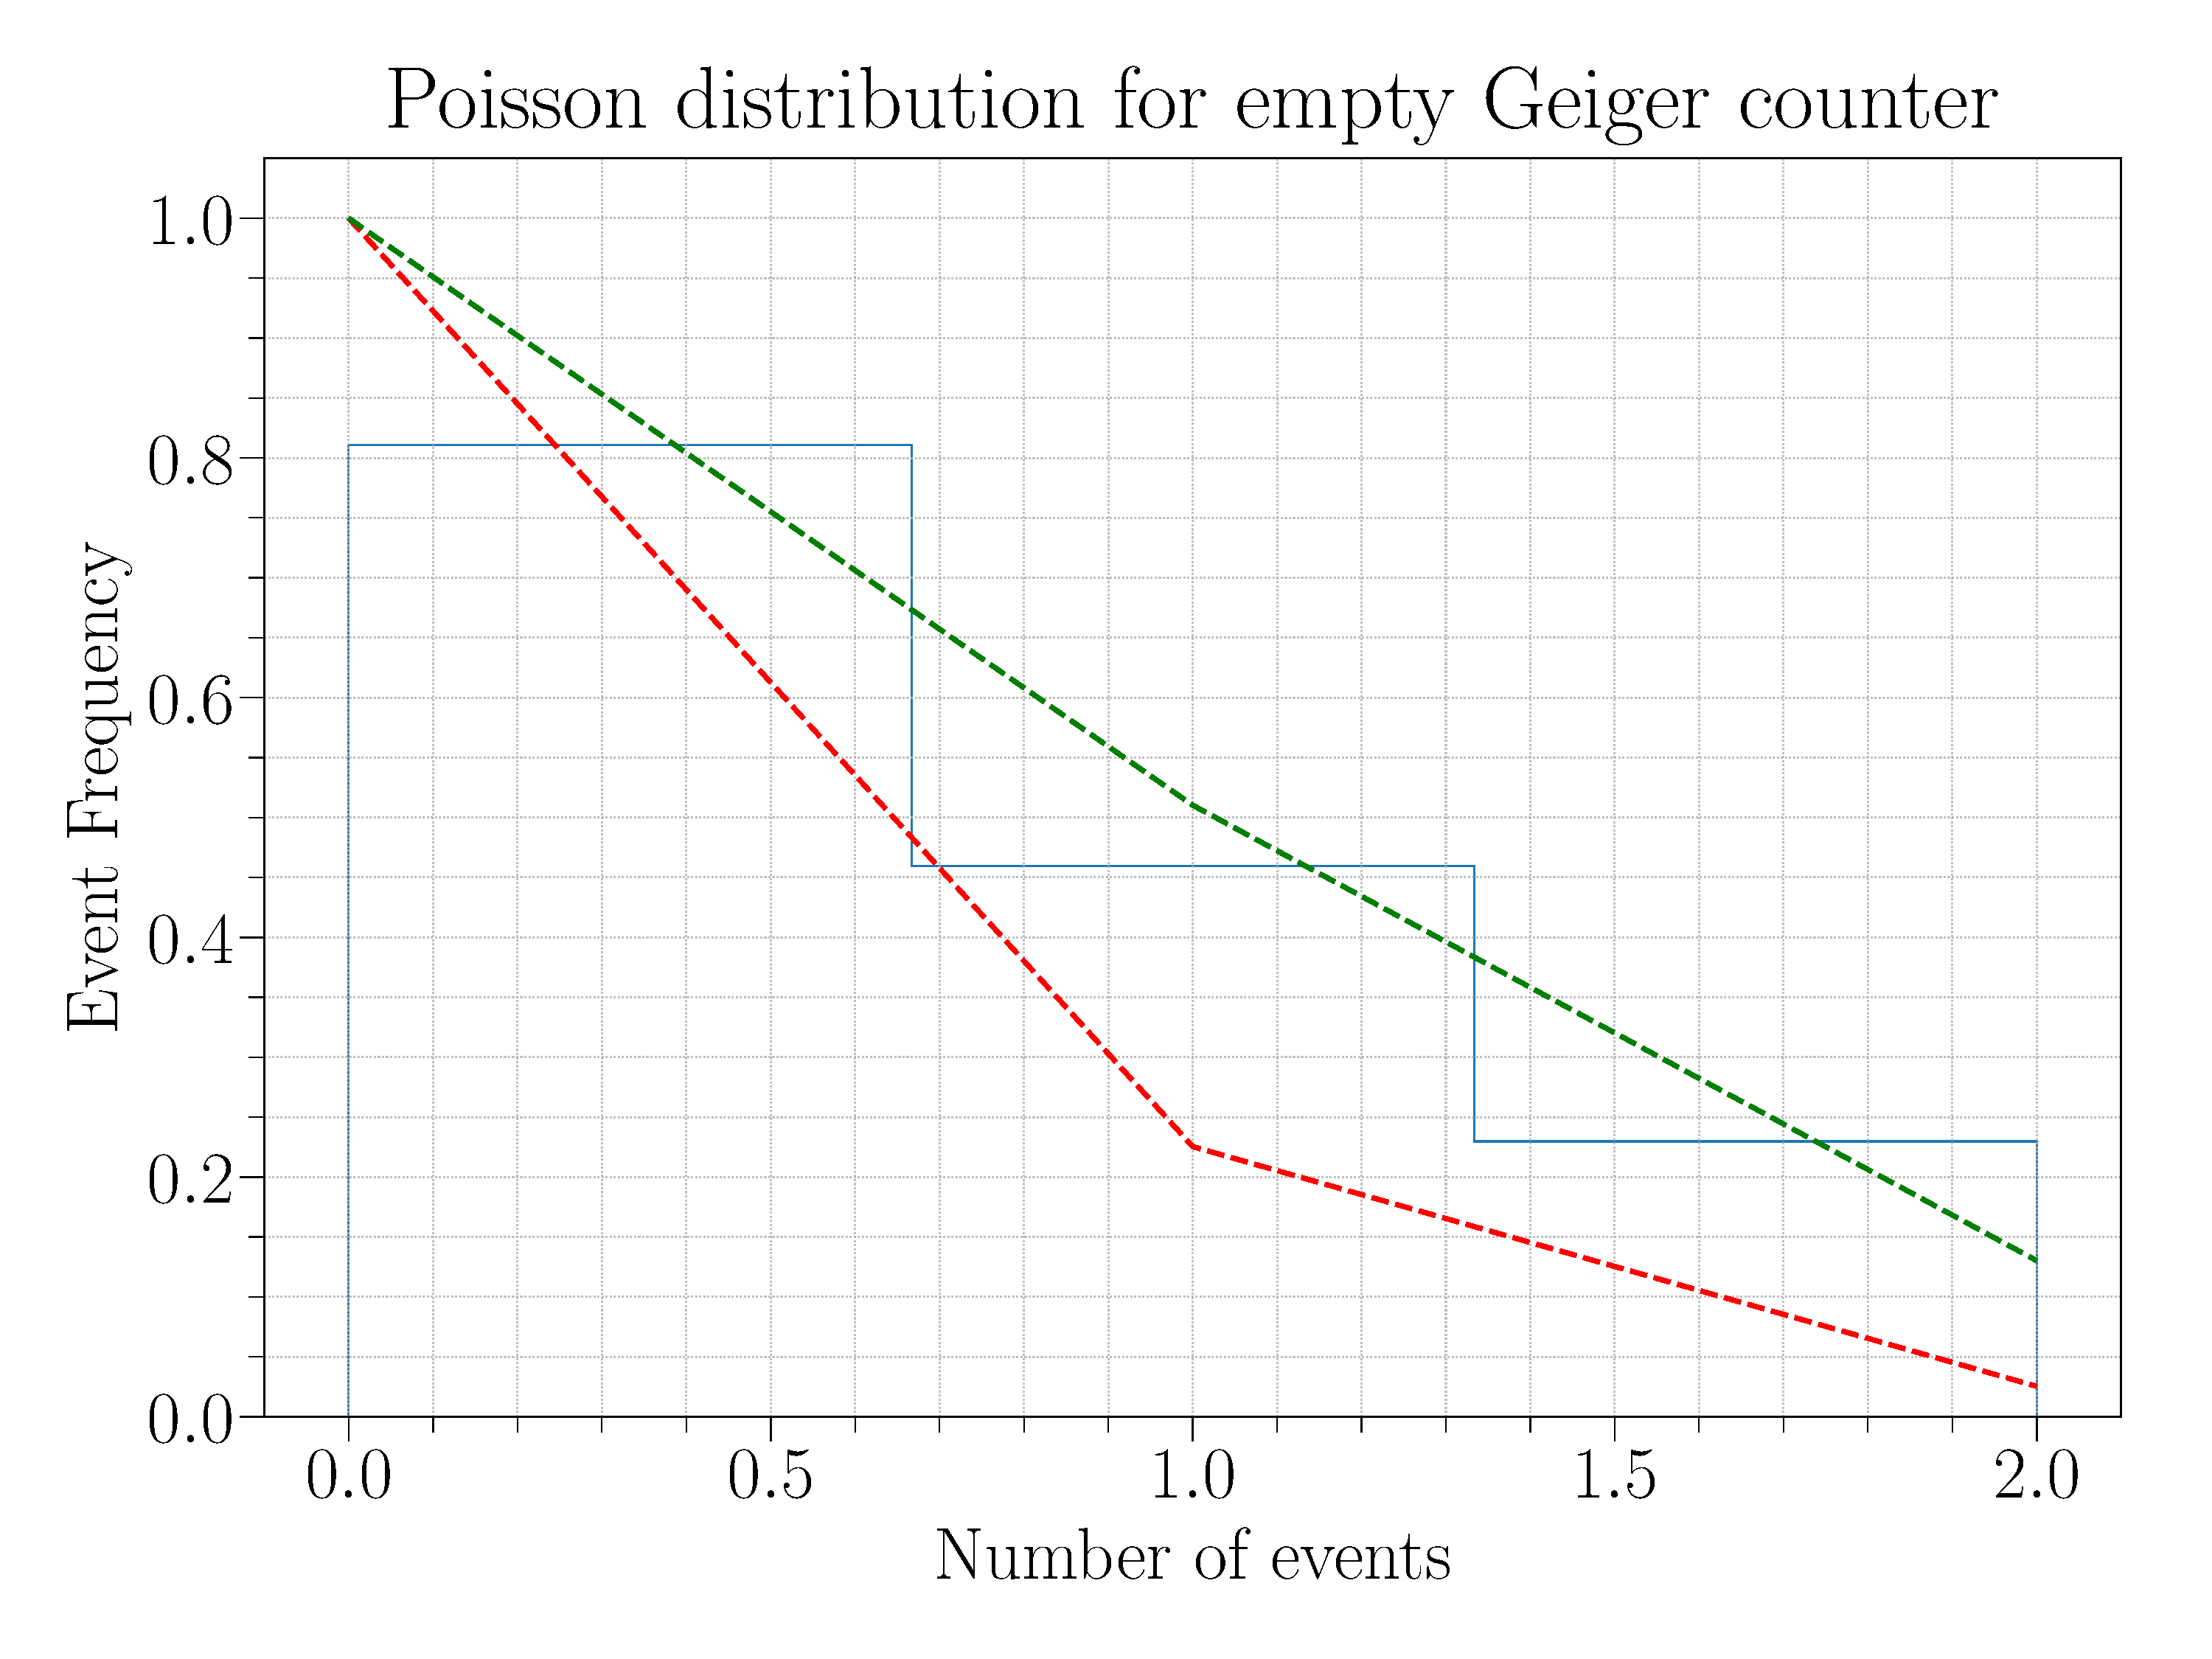
\includegraphics[width=0.9\textwidth]{../Figures/Geiger_poisson_fit.pdf}
\caption{Normalized histogram with expected and fitted poisson distributions.}
\label{fig:PoissonFit}
\end{figure}

\subsubsection{Exponential distribution}

The times between the Poisson-distributed counts should follow a exponential distribution. To test this, we recorded a signal trace of 0.5 s length using the oscilloscope. With the help of the Python-module \code{peakutils} we search for the peaks in the signal to detect events. This can be seen in \cref{fig:peaks}. Here we chose a fairly low threshold for the peak height, to account for all possible detections of the external counter, as we do not know its voltage threshold. We were able to detect 106 events in total.

\begin{figure}[h]
	\centering
	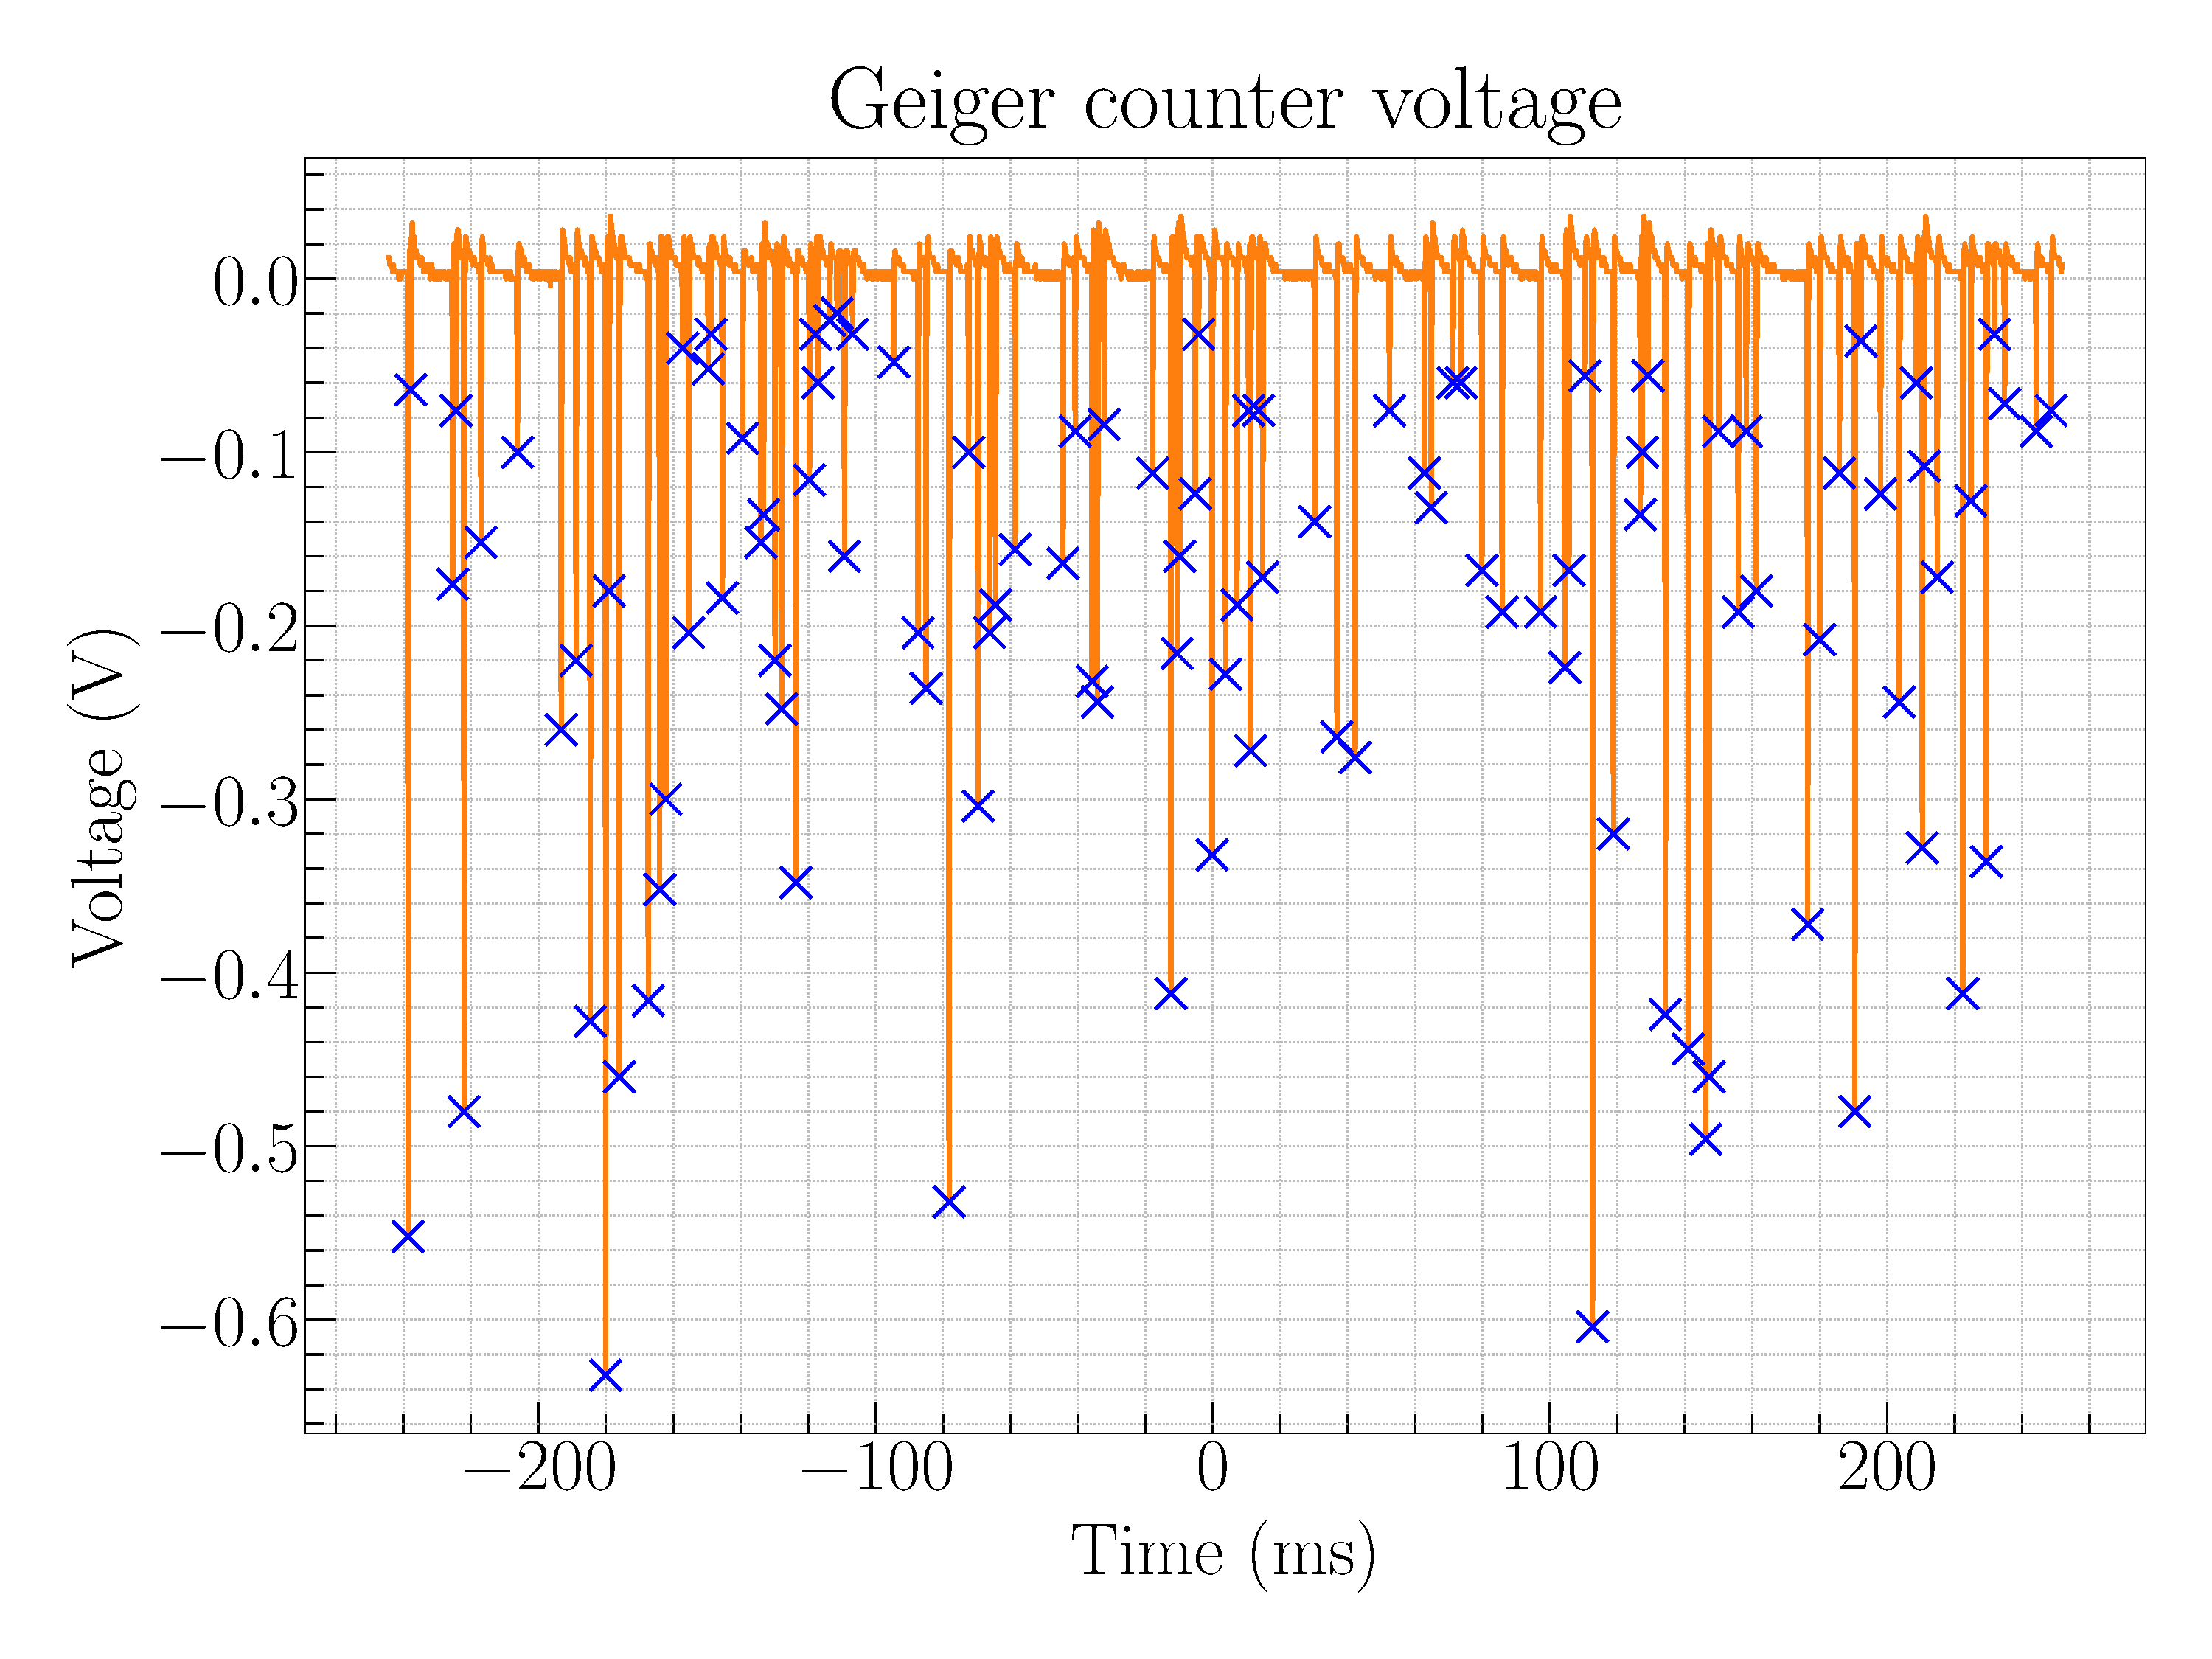
\includegraphics[width=0.9\textwidth]{../Figures/Geiger_peaks_0,5s.pdf}
	\caption{Voltage signal from the GM-counter during 0.5s, with peaks of event detected by a peakfinder.}
	\label{fig:peaks}
\end{figure}

We then proceed to compute the time differences between all the event peaks and plot a histogram of those, seen in \cref{fig:expHist}.

\begin{figure}[H]
\centering
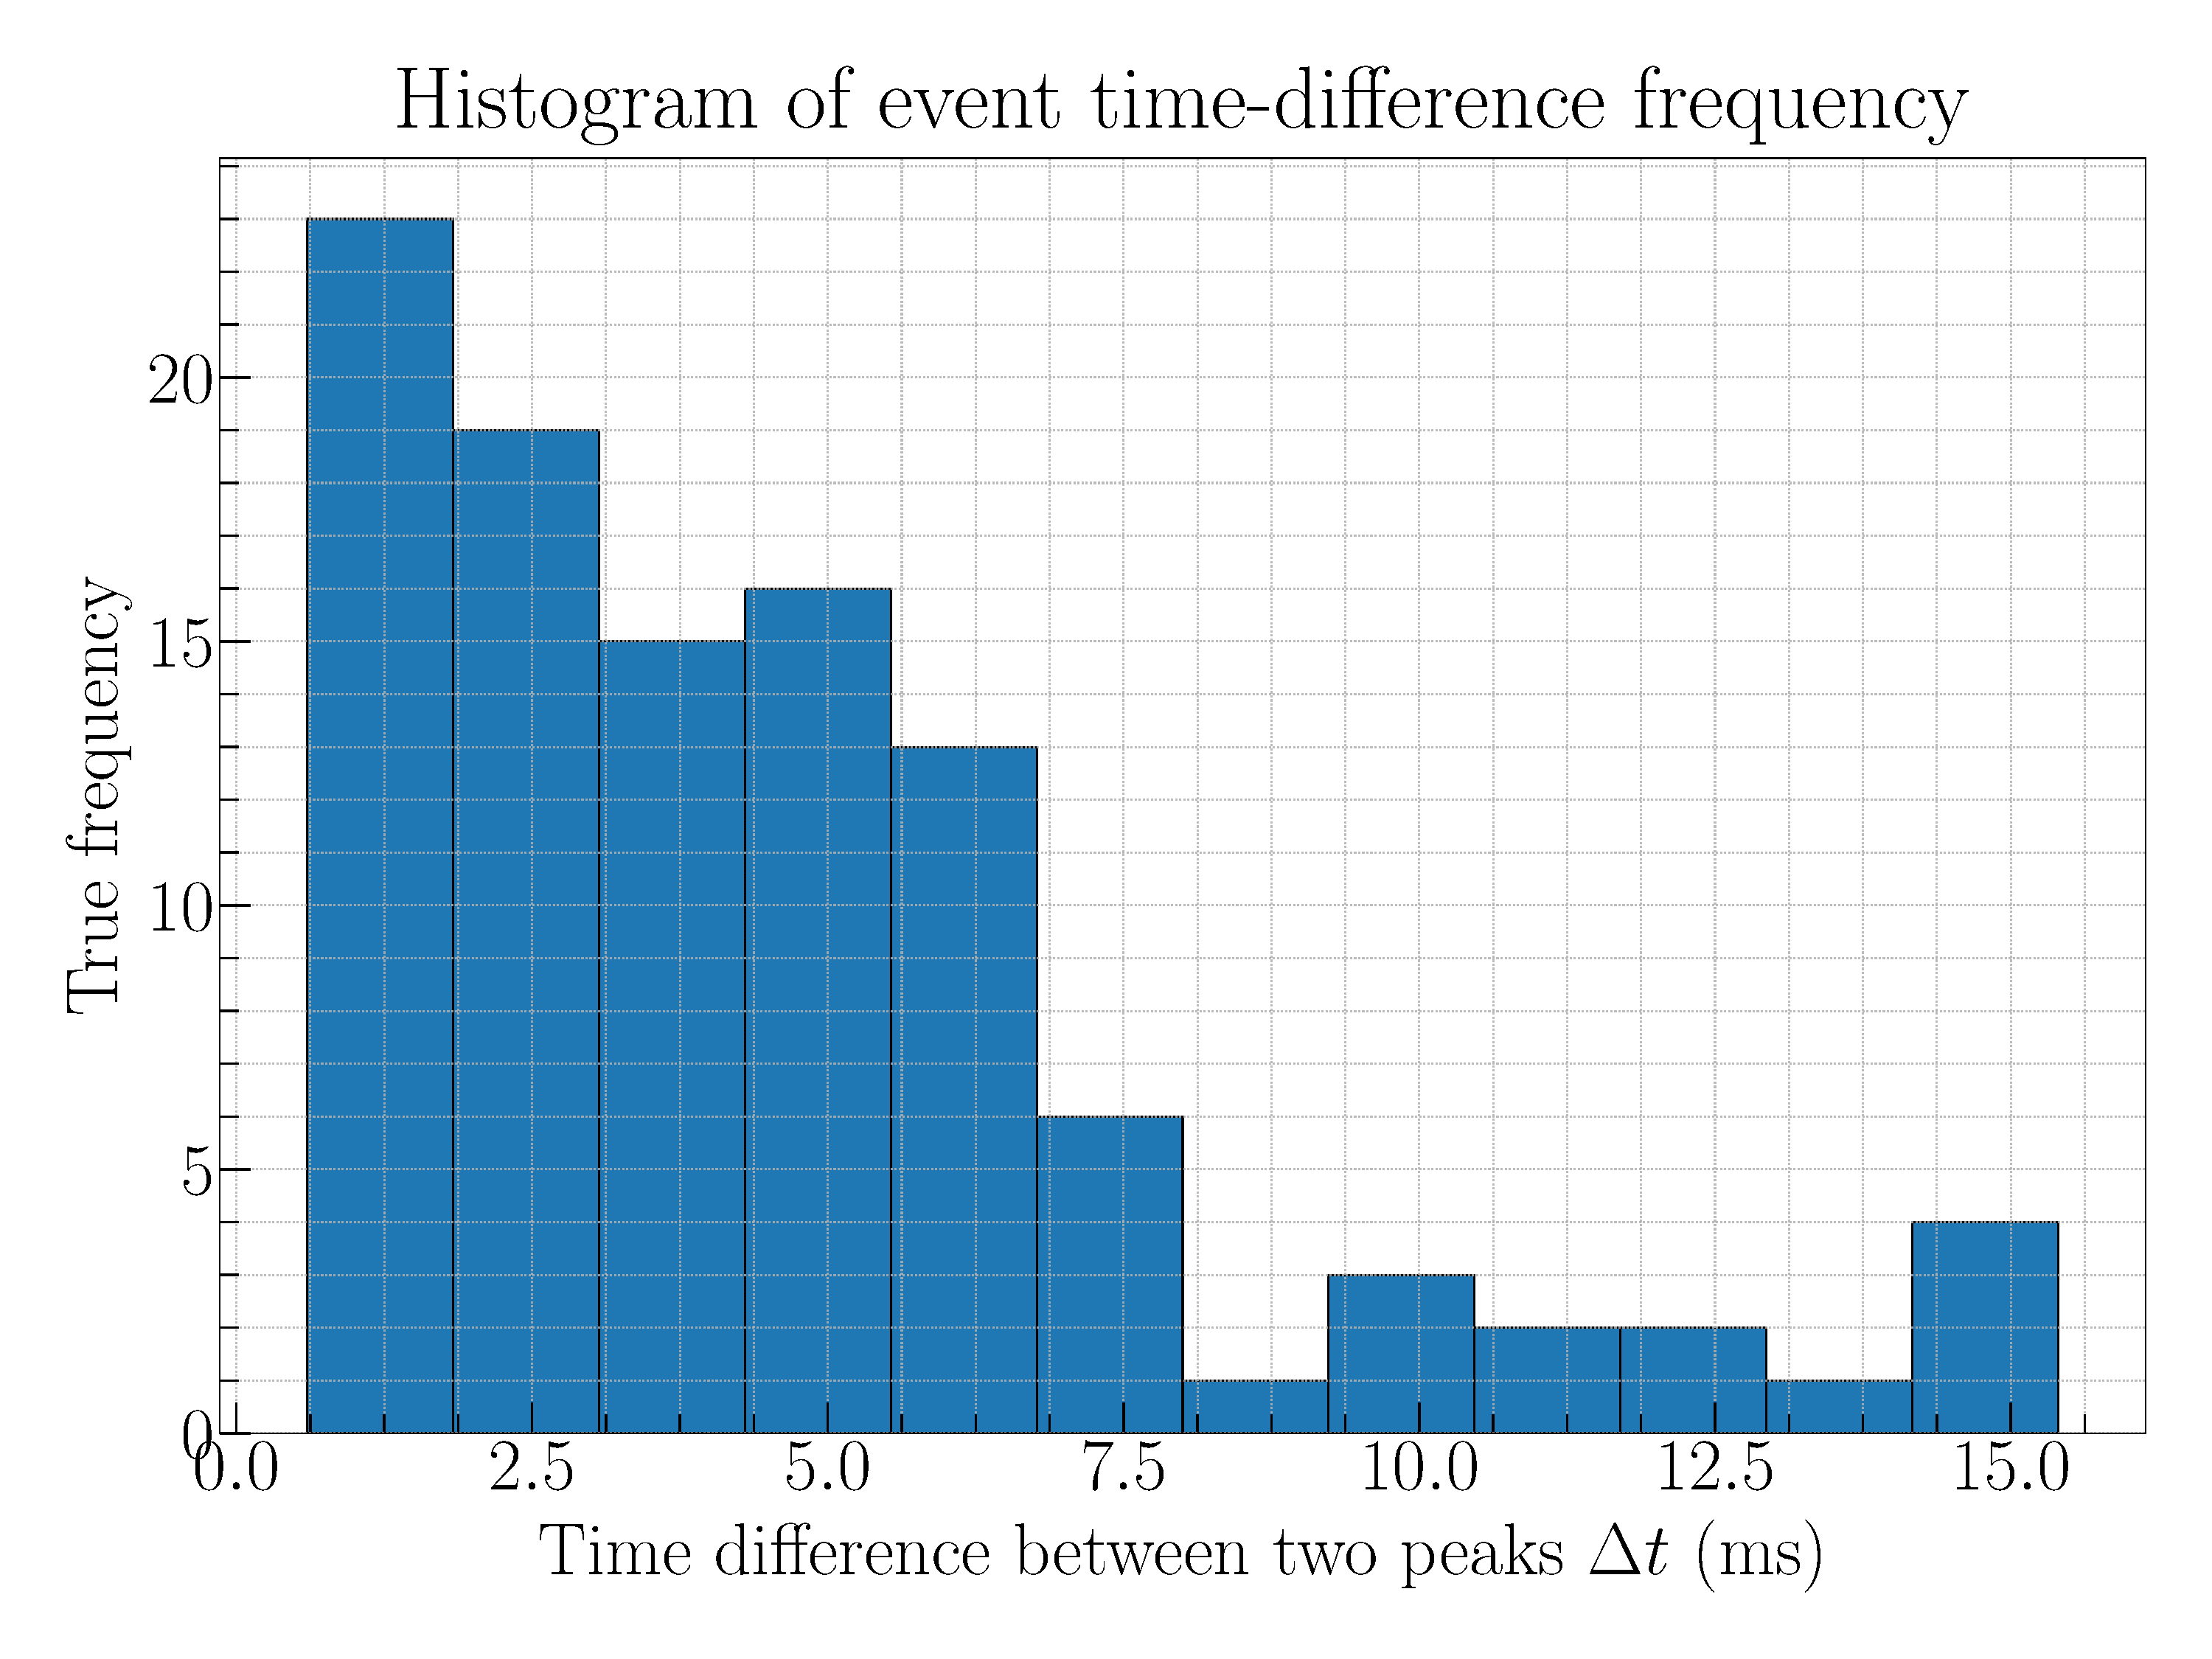
\includegraphics[width=0.9\textwidth]{../Figures/Geiger_eventtime_histogram_unnormalized.pdf}
\caption{Event time histogram}
\label{fig:expHist}
\end{figure}

To actually compare the histogram with the expected and fitted distributions, we normalise it so that the total area is 1.

We estimated the event rate $A$ using two methods: using the computed activity of the sample given in Bequerel (events/second) from \cref{tab:Activity}, and using the peaks shown in \cref{fig:peaks}, which gives us $A = 213.6 $ events/second. Nonetheless, using these values for the exponential distribution was not successful, as the amplitude of the result was much lower than the measured values. Because of this the curves are not visible in \cref{fig:ExpFit}.

We also performed a nonlinear least-squares fit of \cref{eq:exp} to the histogram, which worked reasonably well as seen in \cref{fig:ExpFit}. 
The results are compiled in \cref{tab:DistPara}. We think that the resulting p-value can not be quite true, as that would say that our data corresponds perfectly with a exponential distribution, which is hard to believe when looking at the histogram.

\begin{figure}[H]
\centering
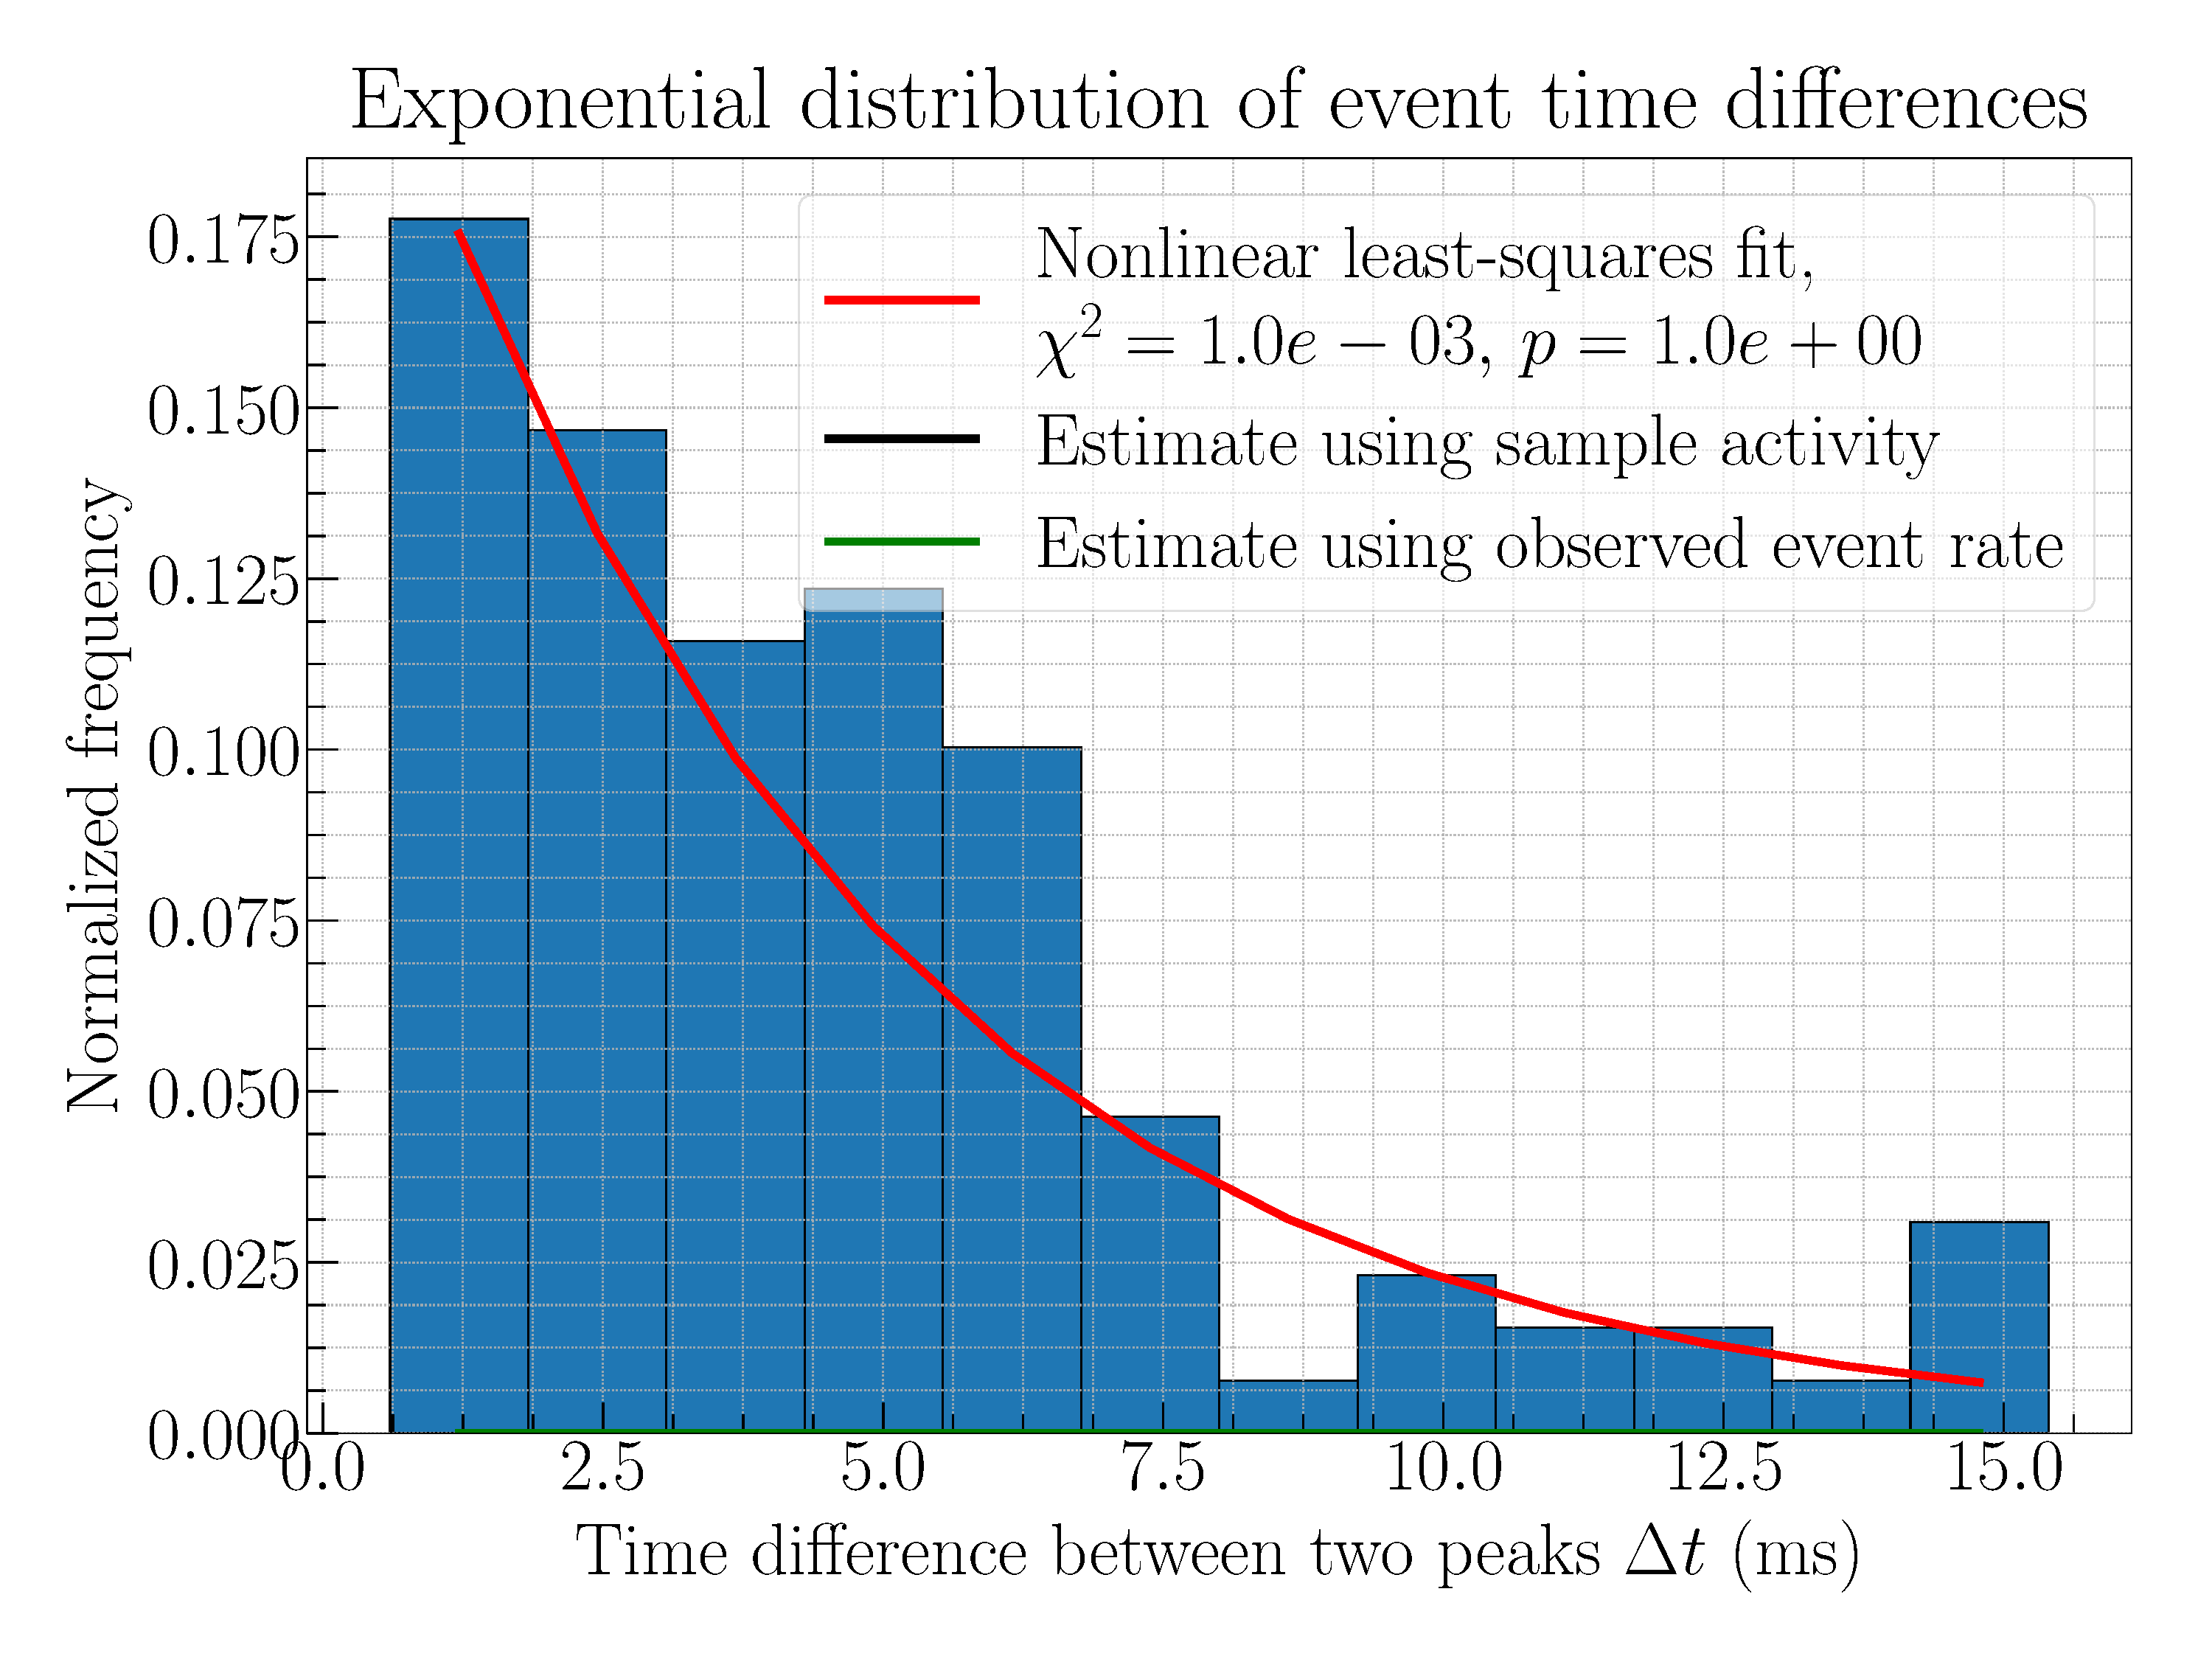
\includegraphics[width=0.9\textwidth]{../Figures/Geiger_eventtime_histogram_fit.pdf}
\caption{Normalized event time histogram with fitted curve. Expected curves are not visible, they turned out to have critically smaller amplitude.}
\label{fig:ExpFit}
\end{figure}

\subsubsection{Results}

To test the goodness of our predictions, we did a $\chi^2$ test for all of the distributions. We only used bins with more than 4 events for the test. The resulting $\chi^2$ and $P$ values are listed in \cref{tab:DistGood}.

\begin{table}[H]
	\renewcommand{\arraystretch}{1.5}
	\centering
	\begin{tabular}{|c|c|c|c|}
		\hline
		Distribution & Parameter & Expected & Fitted \\
		\hline
		\multirow{2}{*}{Gaussian} & $\mu$ & \SI{260.14 \pm 1.14}{} & \SI{260.10 \pm 2.67}{} \\
		 & $\sigma$ & \SI{11.37}{} & \SI{11.51 \pm 1.86}{} \\
		\hline
		\multirow{2}{*}{Poisson} & $\mu$ & \SI{0.66 \pm 0.08}{} & \SI{1.14 \pm 0.20}{} \\
		 & $\sigma = \sqrt{\mu}$ & \SI{0.81 \pm 0,05}{} & \SI{1,07 \pm 0,10}{} \\
		\hline
		\multirow{2}{*}{Exponential} & $\mu = A^{-1}$ & \SI{0.005}{s} & \SI{4.3+-0.9}{s} \\
		 & $\sigma  = A^{-1} $ & \SI{0.005}{s} & \SI{4.3+-0.9}{s} \\
		\hline
	\end{tabular}
	\caption{Parameters for expected and fitted distributions.}
	\label{tab:DistPara}
\end{table}

\begin{table}[H]
	\renewcommand{\arraystretch}{1.5}
	\centering
	\begin{tabular}{|c|c|c|c|}
		\hline
		Distribution & Parameter & Expected & Fitted \\
		\hline
		\multirow{2}{*}{Gaussian} & $\chi^2$ & \SI{0.115}{} & \SI{0.119}{} \\
		 & $P$ value & \SI{0.944}{} & \SI{0.942}{} \\
		\hline
		\multirow{2}{*}{Poisson} & $\chi^2$ & \SI{1.02}{} & \SI{0.23}{} \\
		 & $P$ value & \SI{0.31}{} & \SI{0.63}{} \\
		\hline
		\multirow{2}{*}{Exponential} & $\chi^2$ & -- & \SI{1e-3}{} \\
		 & $P$ value & -- & \SI{1}{} \\
		\hline
	\end{tabular}
	\caption{Goodness of expected and fitted distributions.}
	\label{tab:DistGood}
\end{table}

\section{Measurements with the proportional counter}

\subsection{Setup}

\begin{figure}[H]
	\centering
	\includegraphics[width=\textwidth]{IMG_20190314_162917.jpg}
	\caption{The setup with the proportional counter on the left, connected to oscilloscope and digital counter}
	\label{fig:}
\end{figure}

The methan-gas-flow proportional counter is flushed continuously with a argon-methan mixture. We will analyse a Am241, as well as a C14 probe. The activity of the sources on the day of the experiment is shown in \cref{tab:Activity}. When used, the probes are placed inside a sample changer. The electronic setup is equivalent to the one for the Geiger counter.

\subsection{Procedure}

First we insert the Am241-probe inside the sample changer and proceed to measure the pulse rate as a function of the voltage. For each voltage, we also write down the puls heights, which we get from the oscilloscope. Based on their fluctuation we assumed a global error of \SI{2}{mV}.

We repeat the same measurement with the C14-probe and with an empty sample changer.

\subsection{Analysis}

To plot the characteristic curve we use a logarithmic scale, since the range of the count rates stretches over several orders of magnitude. This scale allows us to clearly see the $\alpha$-plateau and the $(\alpha+\beta)$-plateau.

In the curve of the C14 sample we see only the $\alpha$-plateau, as expected because it does not emit $\beta$-radiation.

We assume some correlation between pulse heights and count rates, which is best visible for carbon sample. There the pulse are of constant height during the plateau, and have a significant jump at the same voltage where a jump in count rate is also observed.

For the first plateau in the Am data it is also visible fairly well that pulse height remains constant.

\begin{figure}[H]
\centering
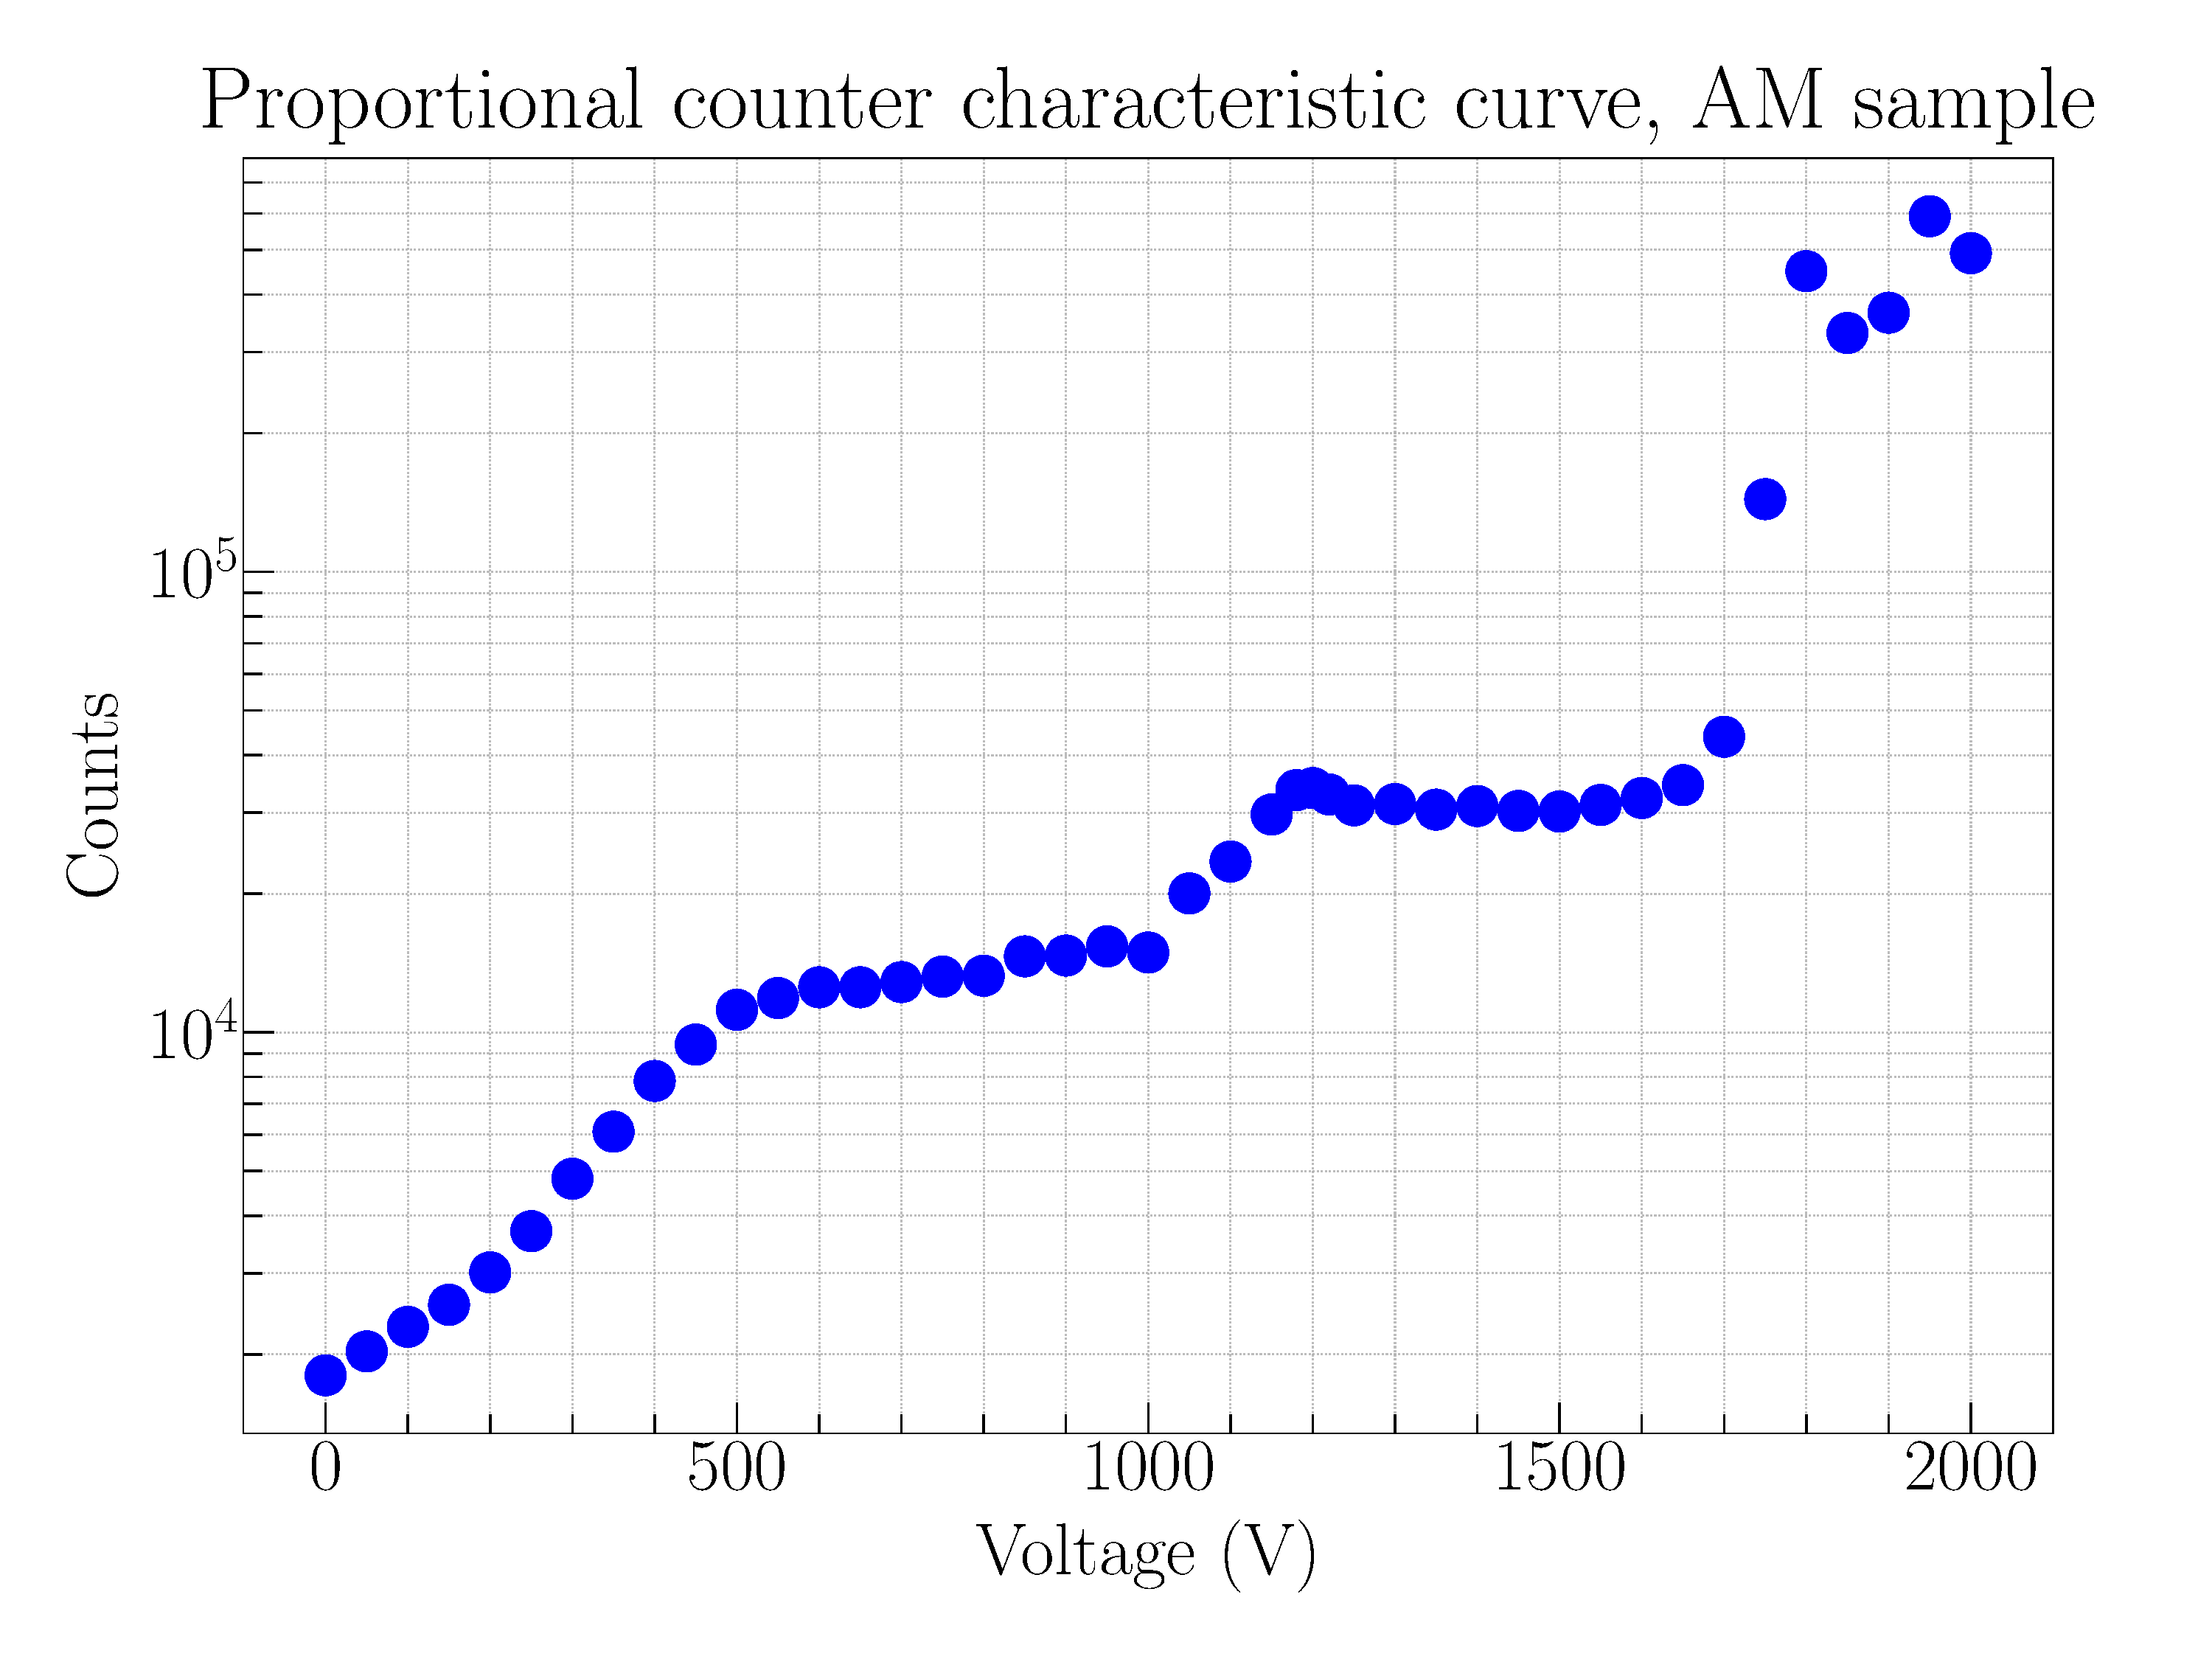
\includegraphics[width=0.8\textwidth]{../Figures/Proportional_characteristic_curve_AM.pdf}
\caption{Characteristic curve with Am plotted on a logarithmic scale. The two plateaus are clearly visible.}
\label{fig:AmChar}
\end{figure}

\begin{figure}[H]
\centering
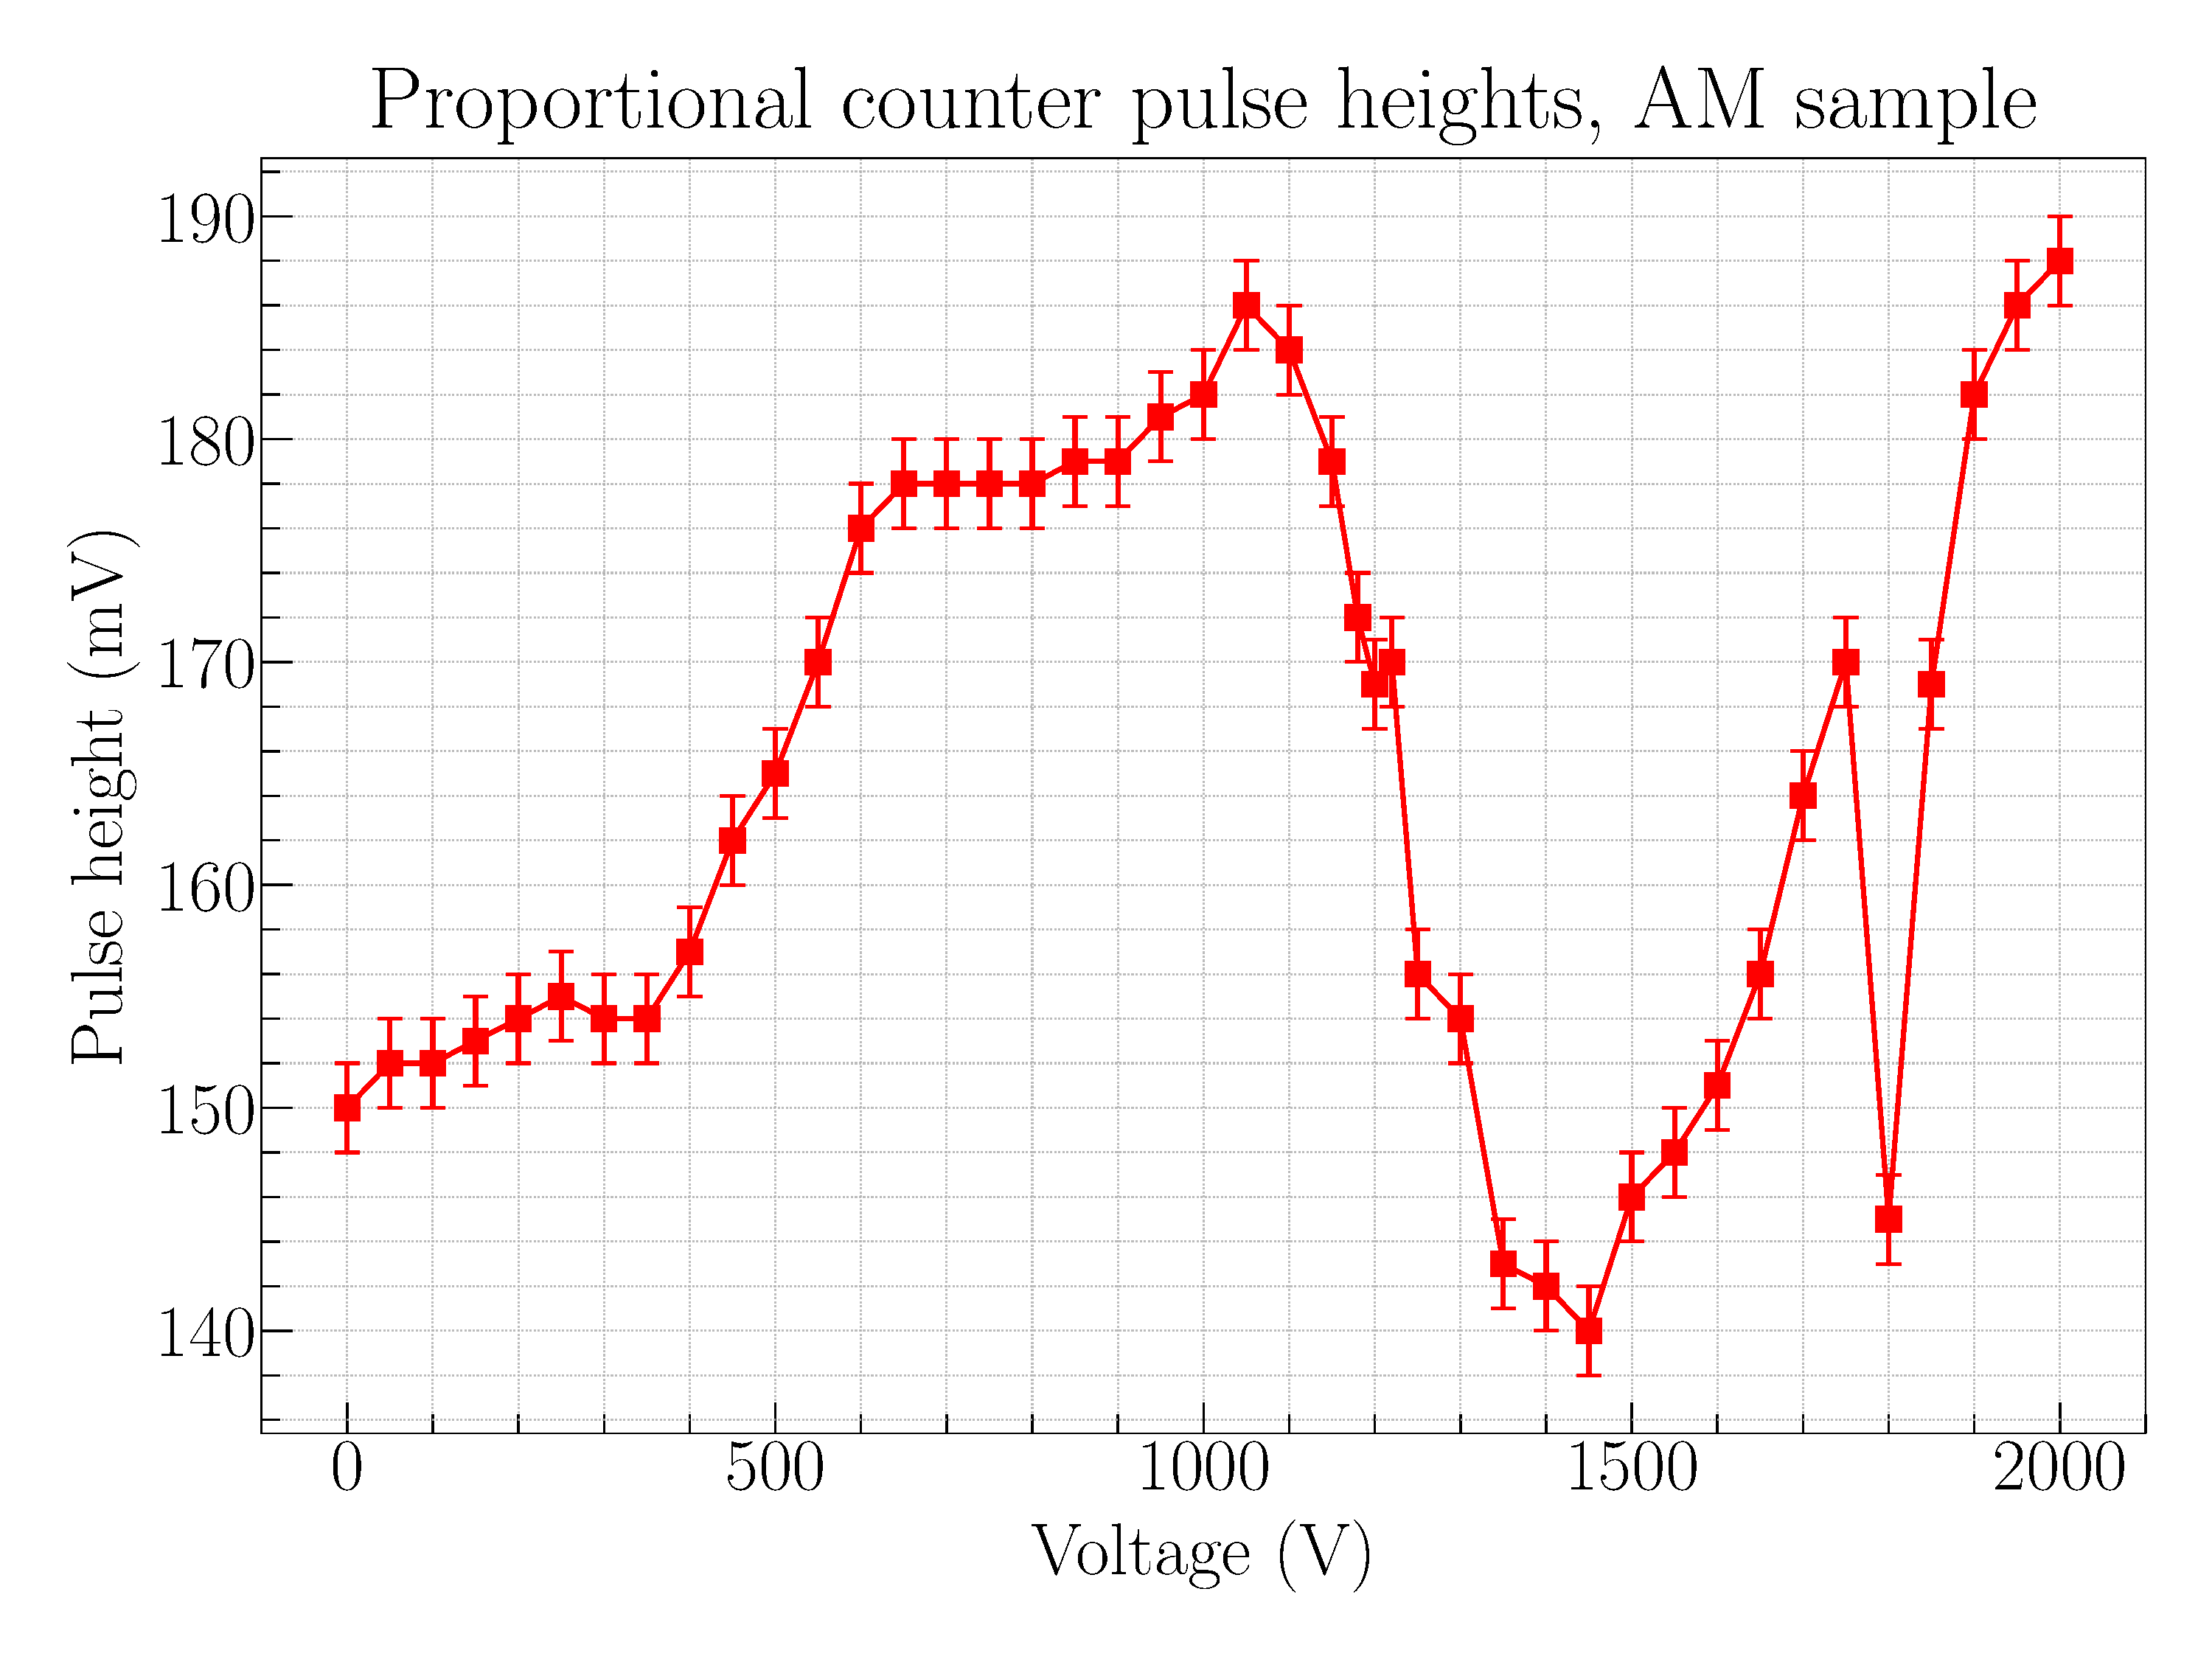
\includegraphics[width=0.8\textwidth]{../Figures/Proportional_pulse_heights_AM.pdf}
\caption{Pulse heights versus voltage for Am. Error bars are due to fluctuations of pulse heights, which were generally in the realm of 2 mV.}
\label{fig:AmPH}
\end{figure}

\begin{figure}[H]
\centering
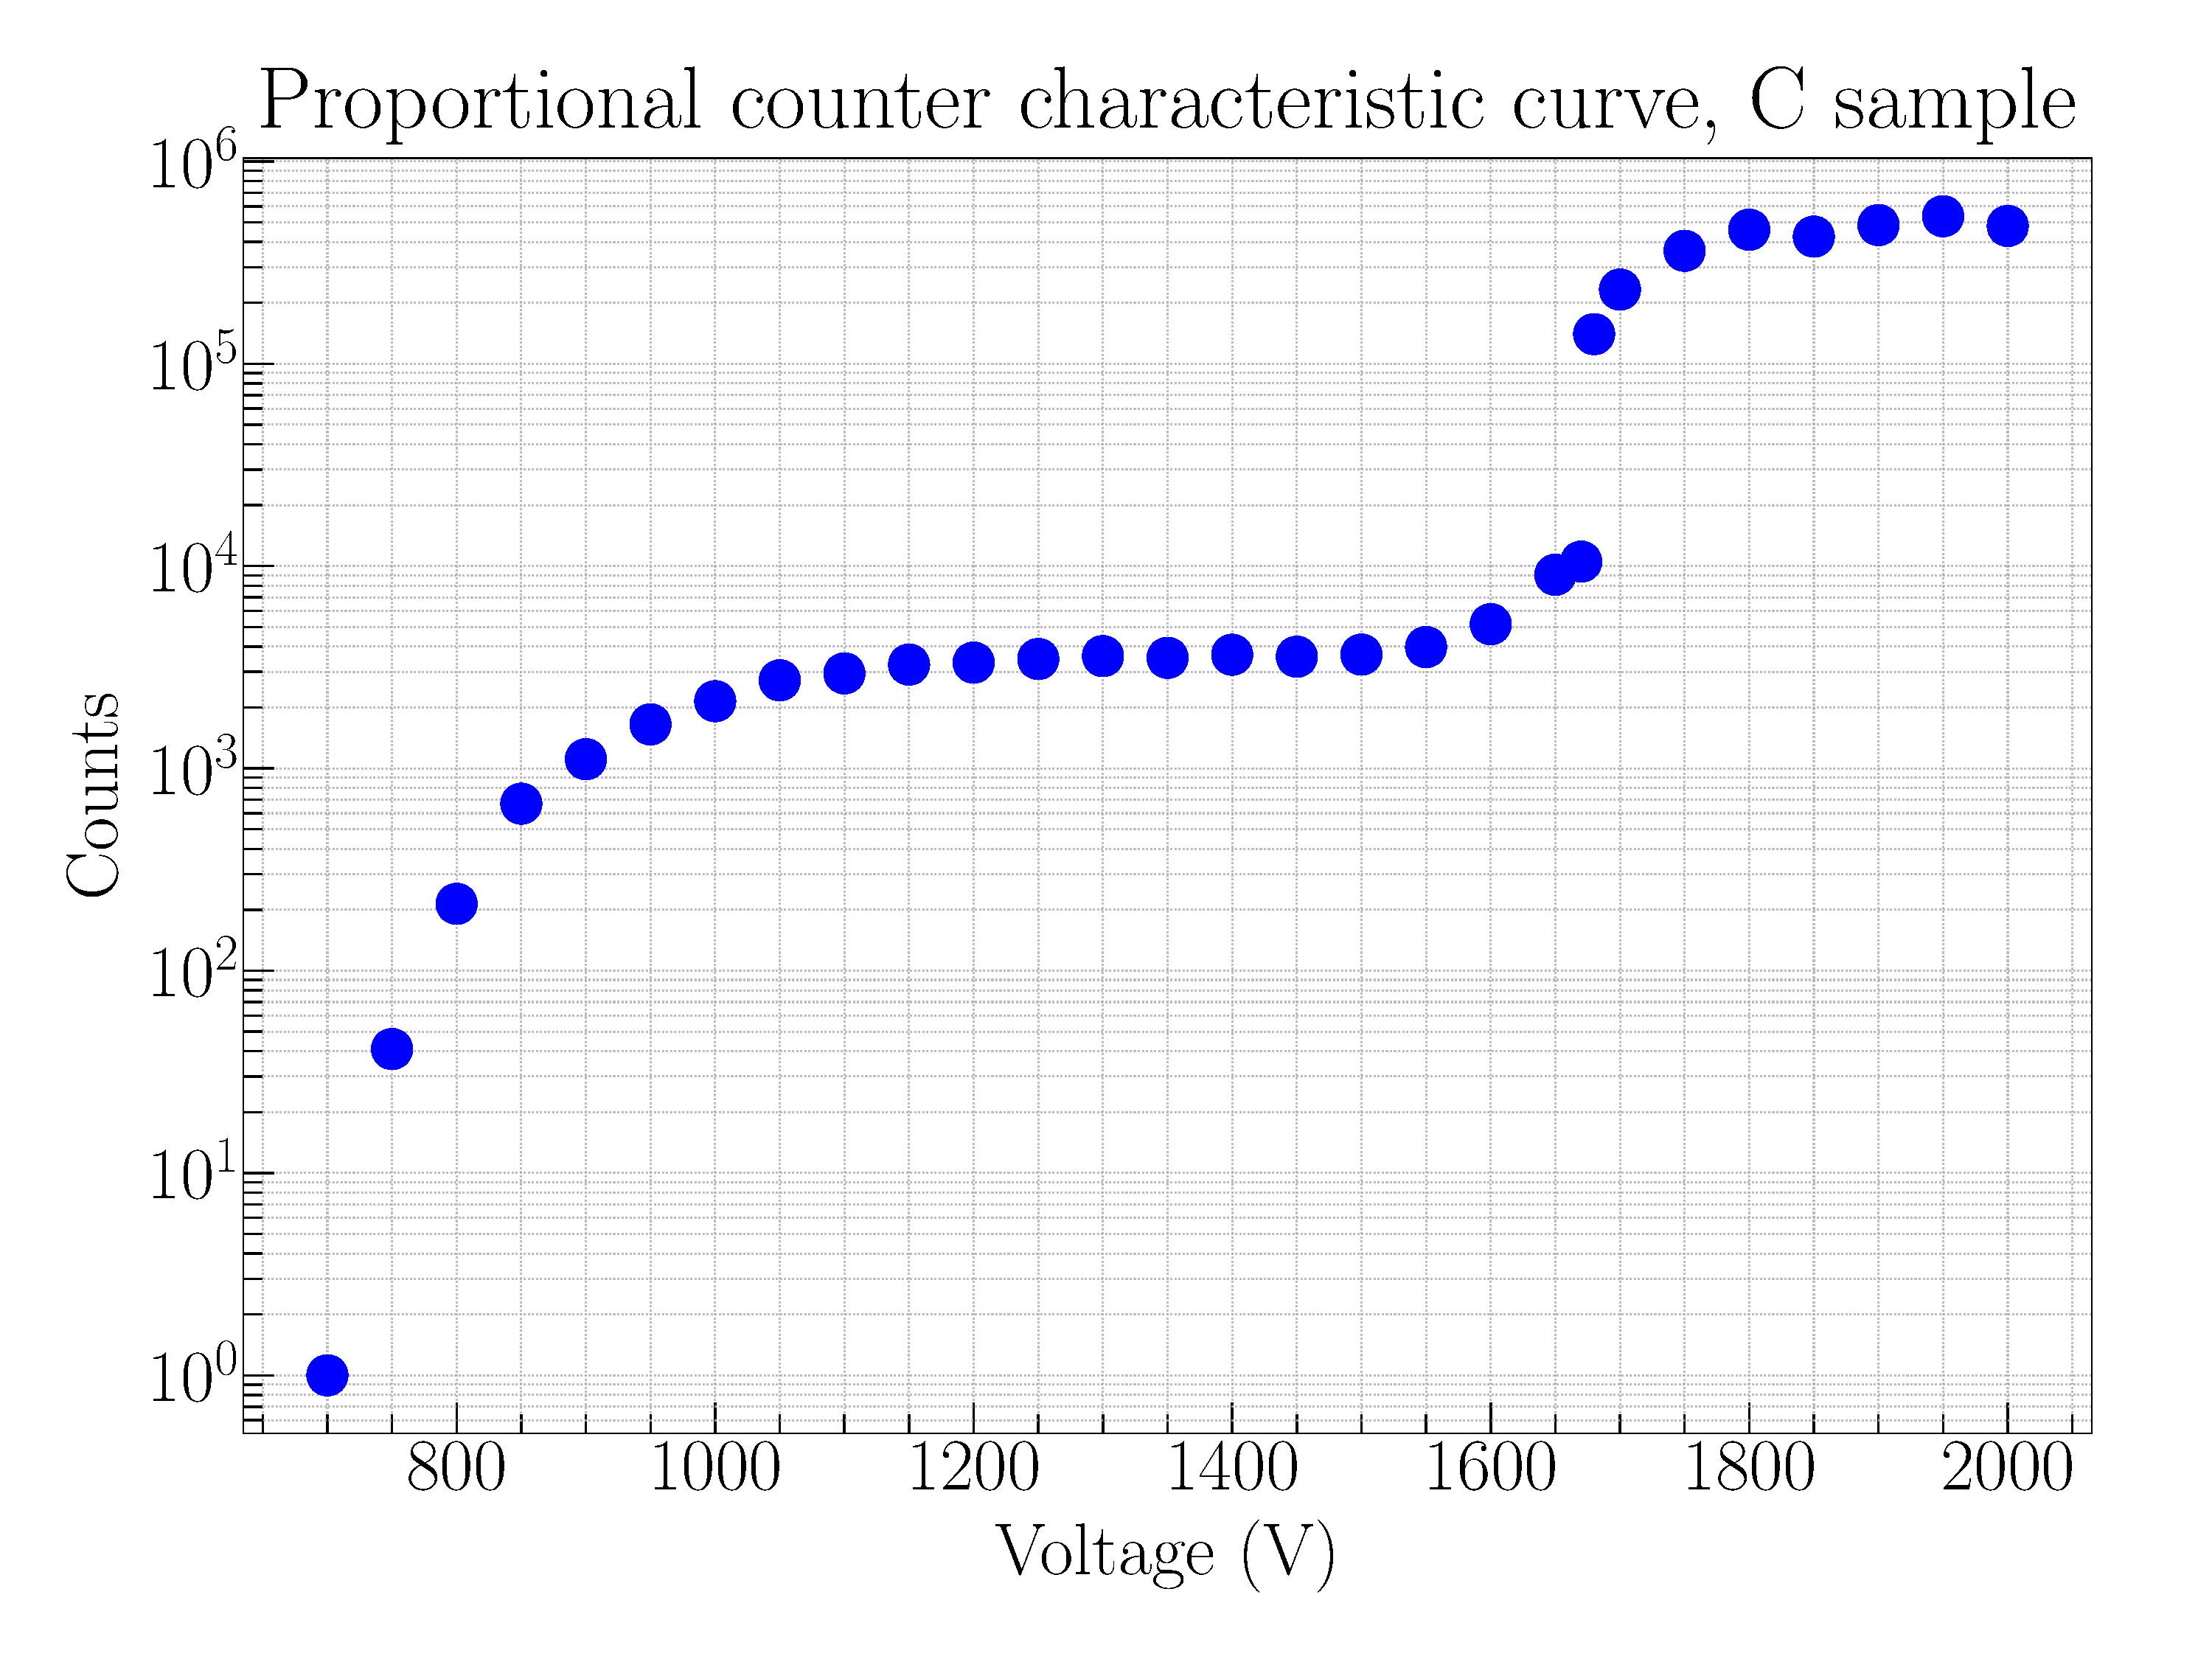
\includegraphics[width=0.8\textwidth]{../Figures/Proportional_characteristic_curve_C.pdf}
\caption{Characteristic curve with C.}
\label{fig:CChar}
\end{figure}

\begin{figure}[H]
\centering
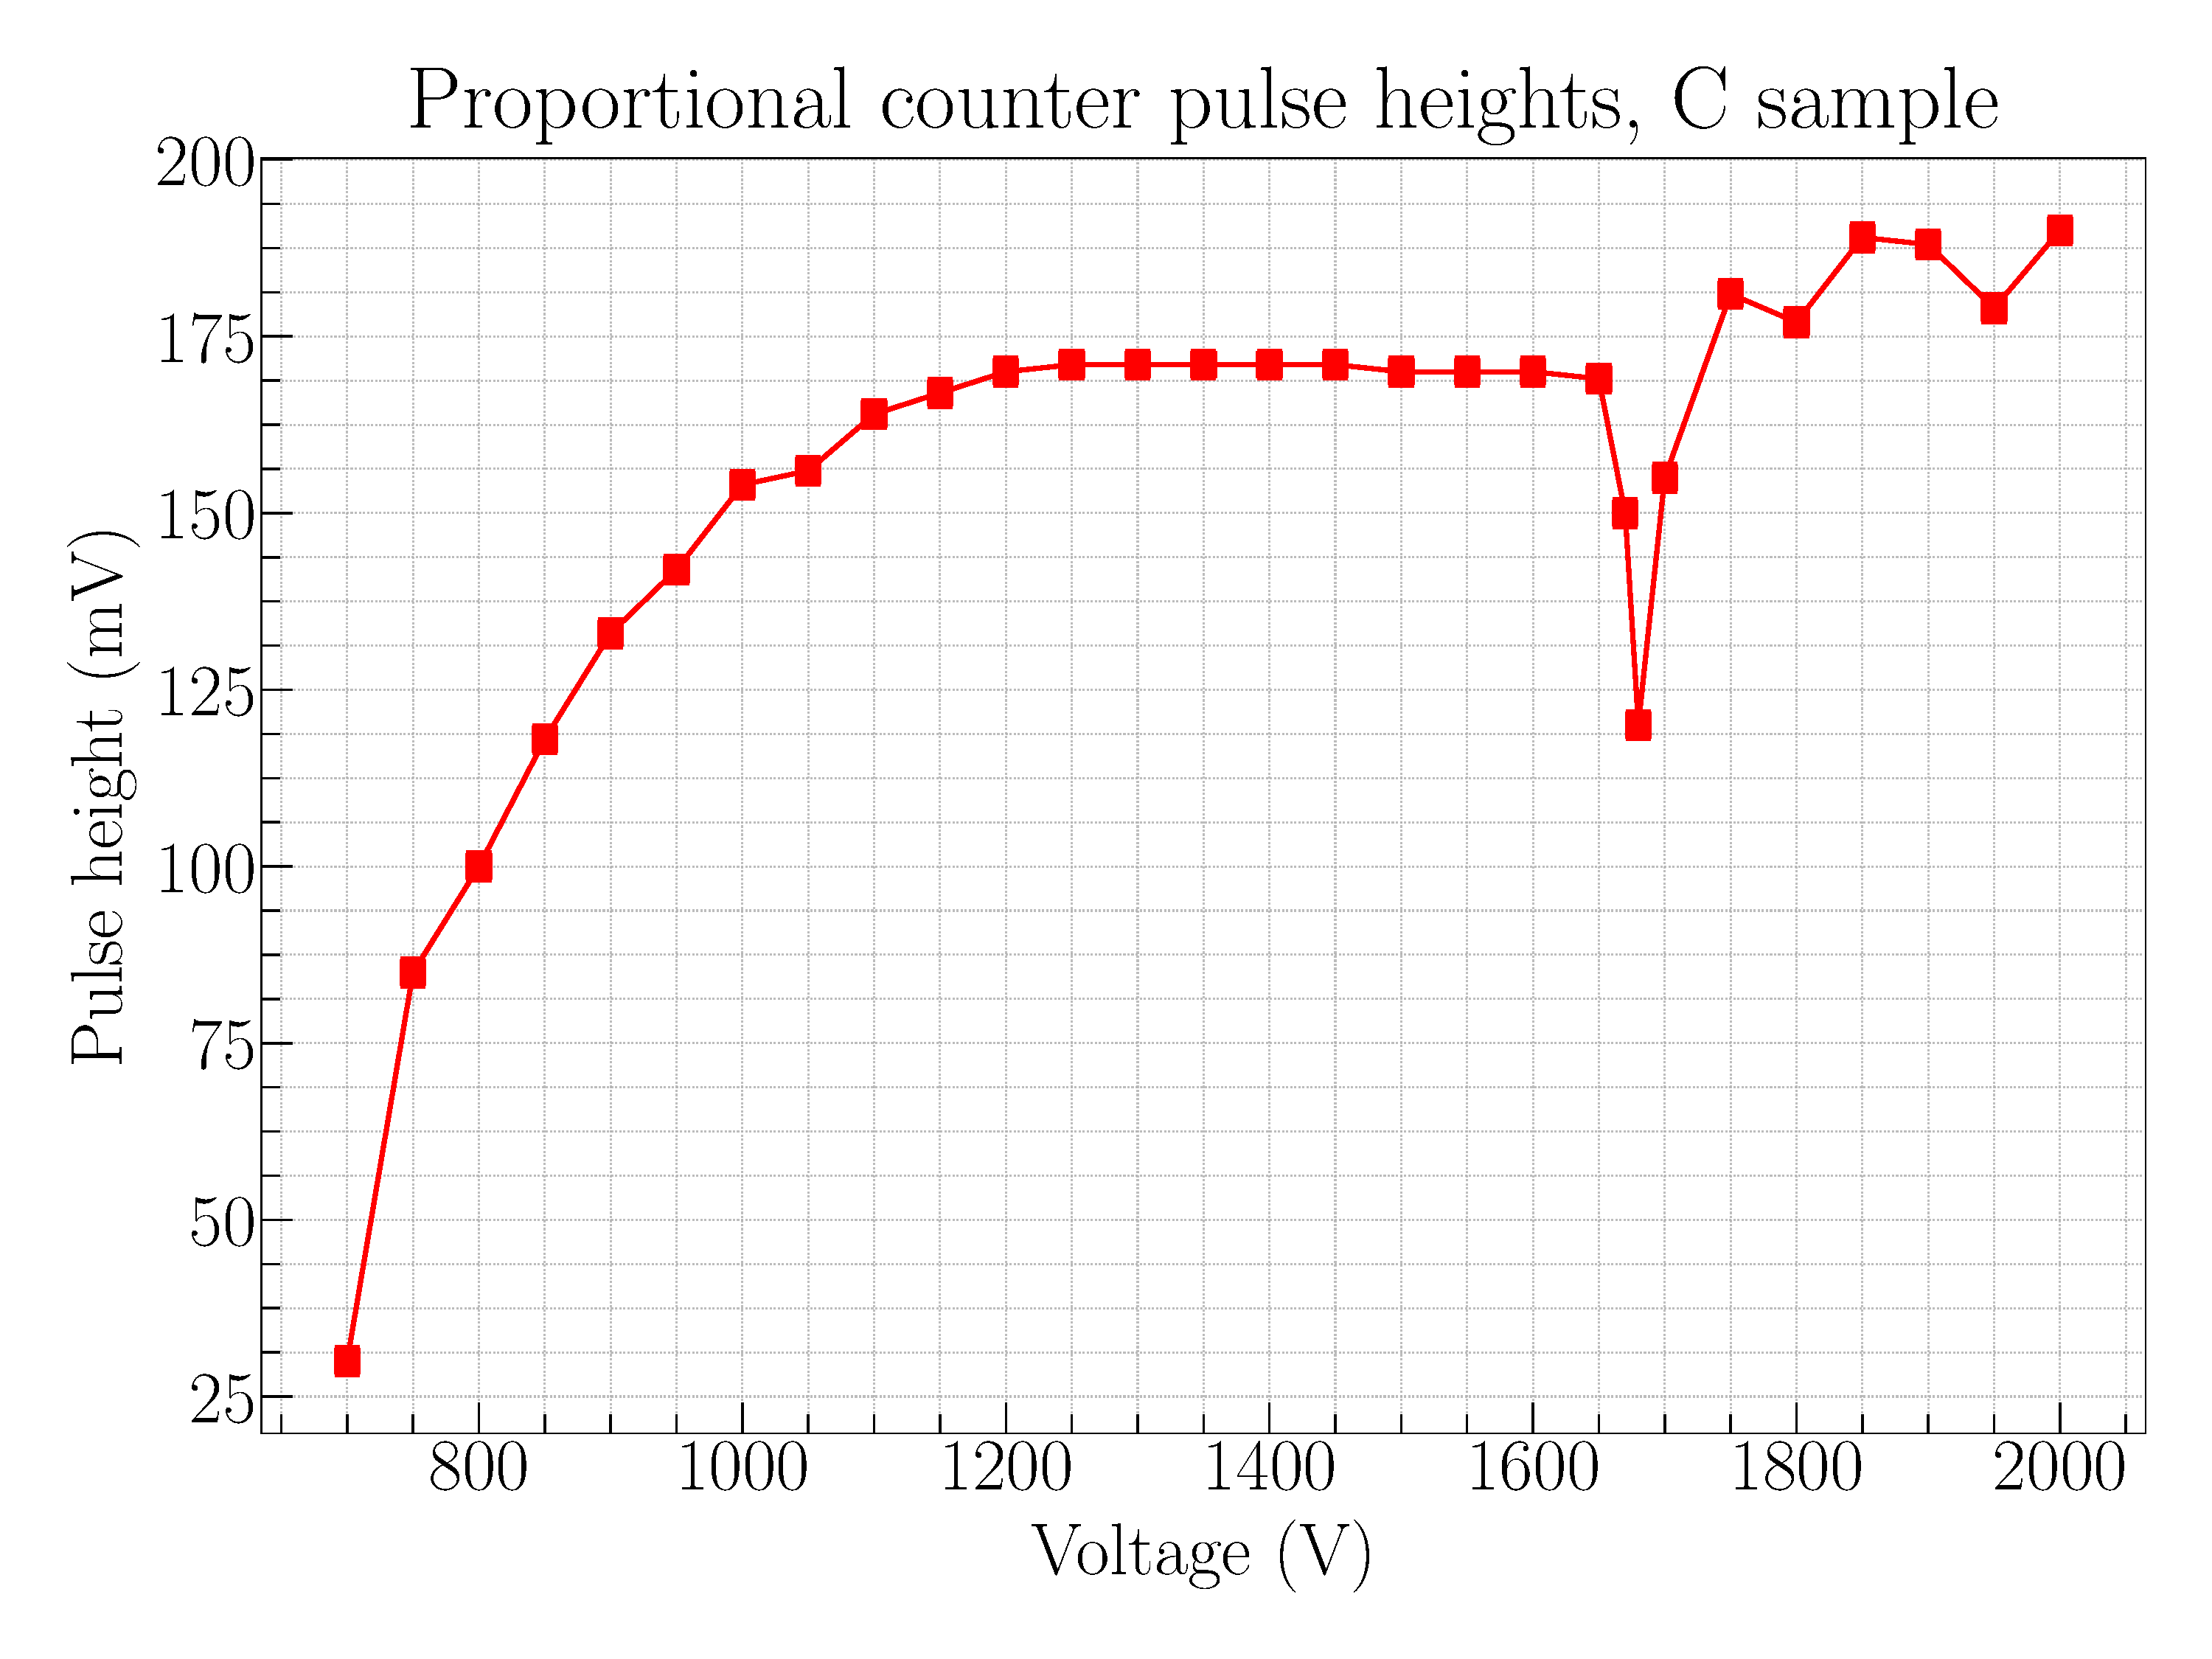
\includegraphics[width=0.8\textwidth]{../Figures/Proportional_pulse_heights_C.pdf}
\caption{Pulse heights versus voltage for C. Error are same as for the Am sample, but too small to be visible in this plot.}
\label{fig:CPH}
\end{figure}

\begin{figure}[H]
\centering
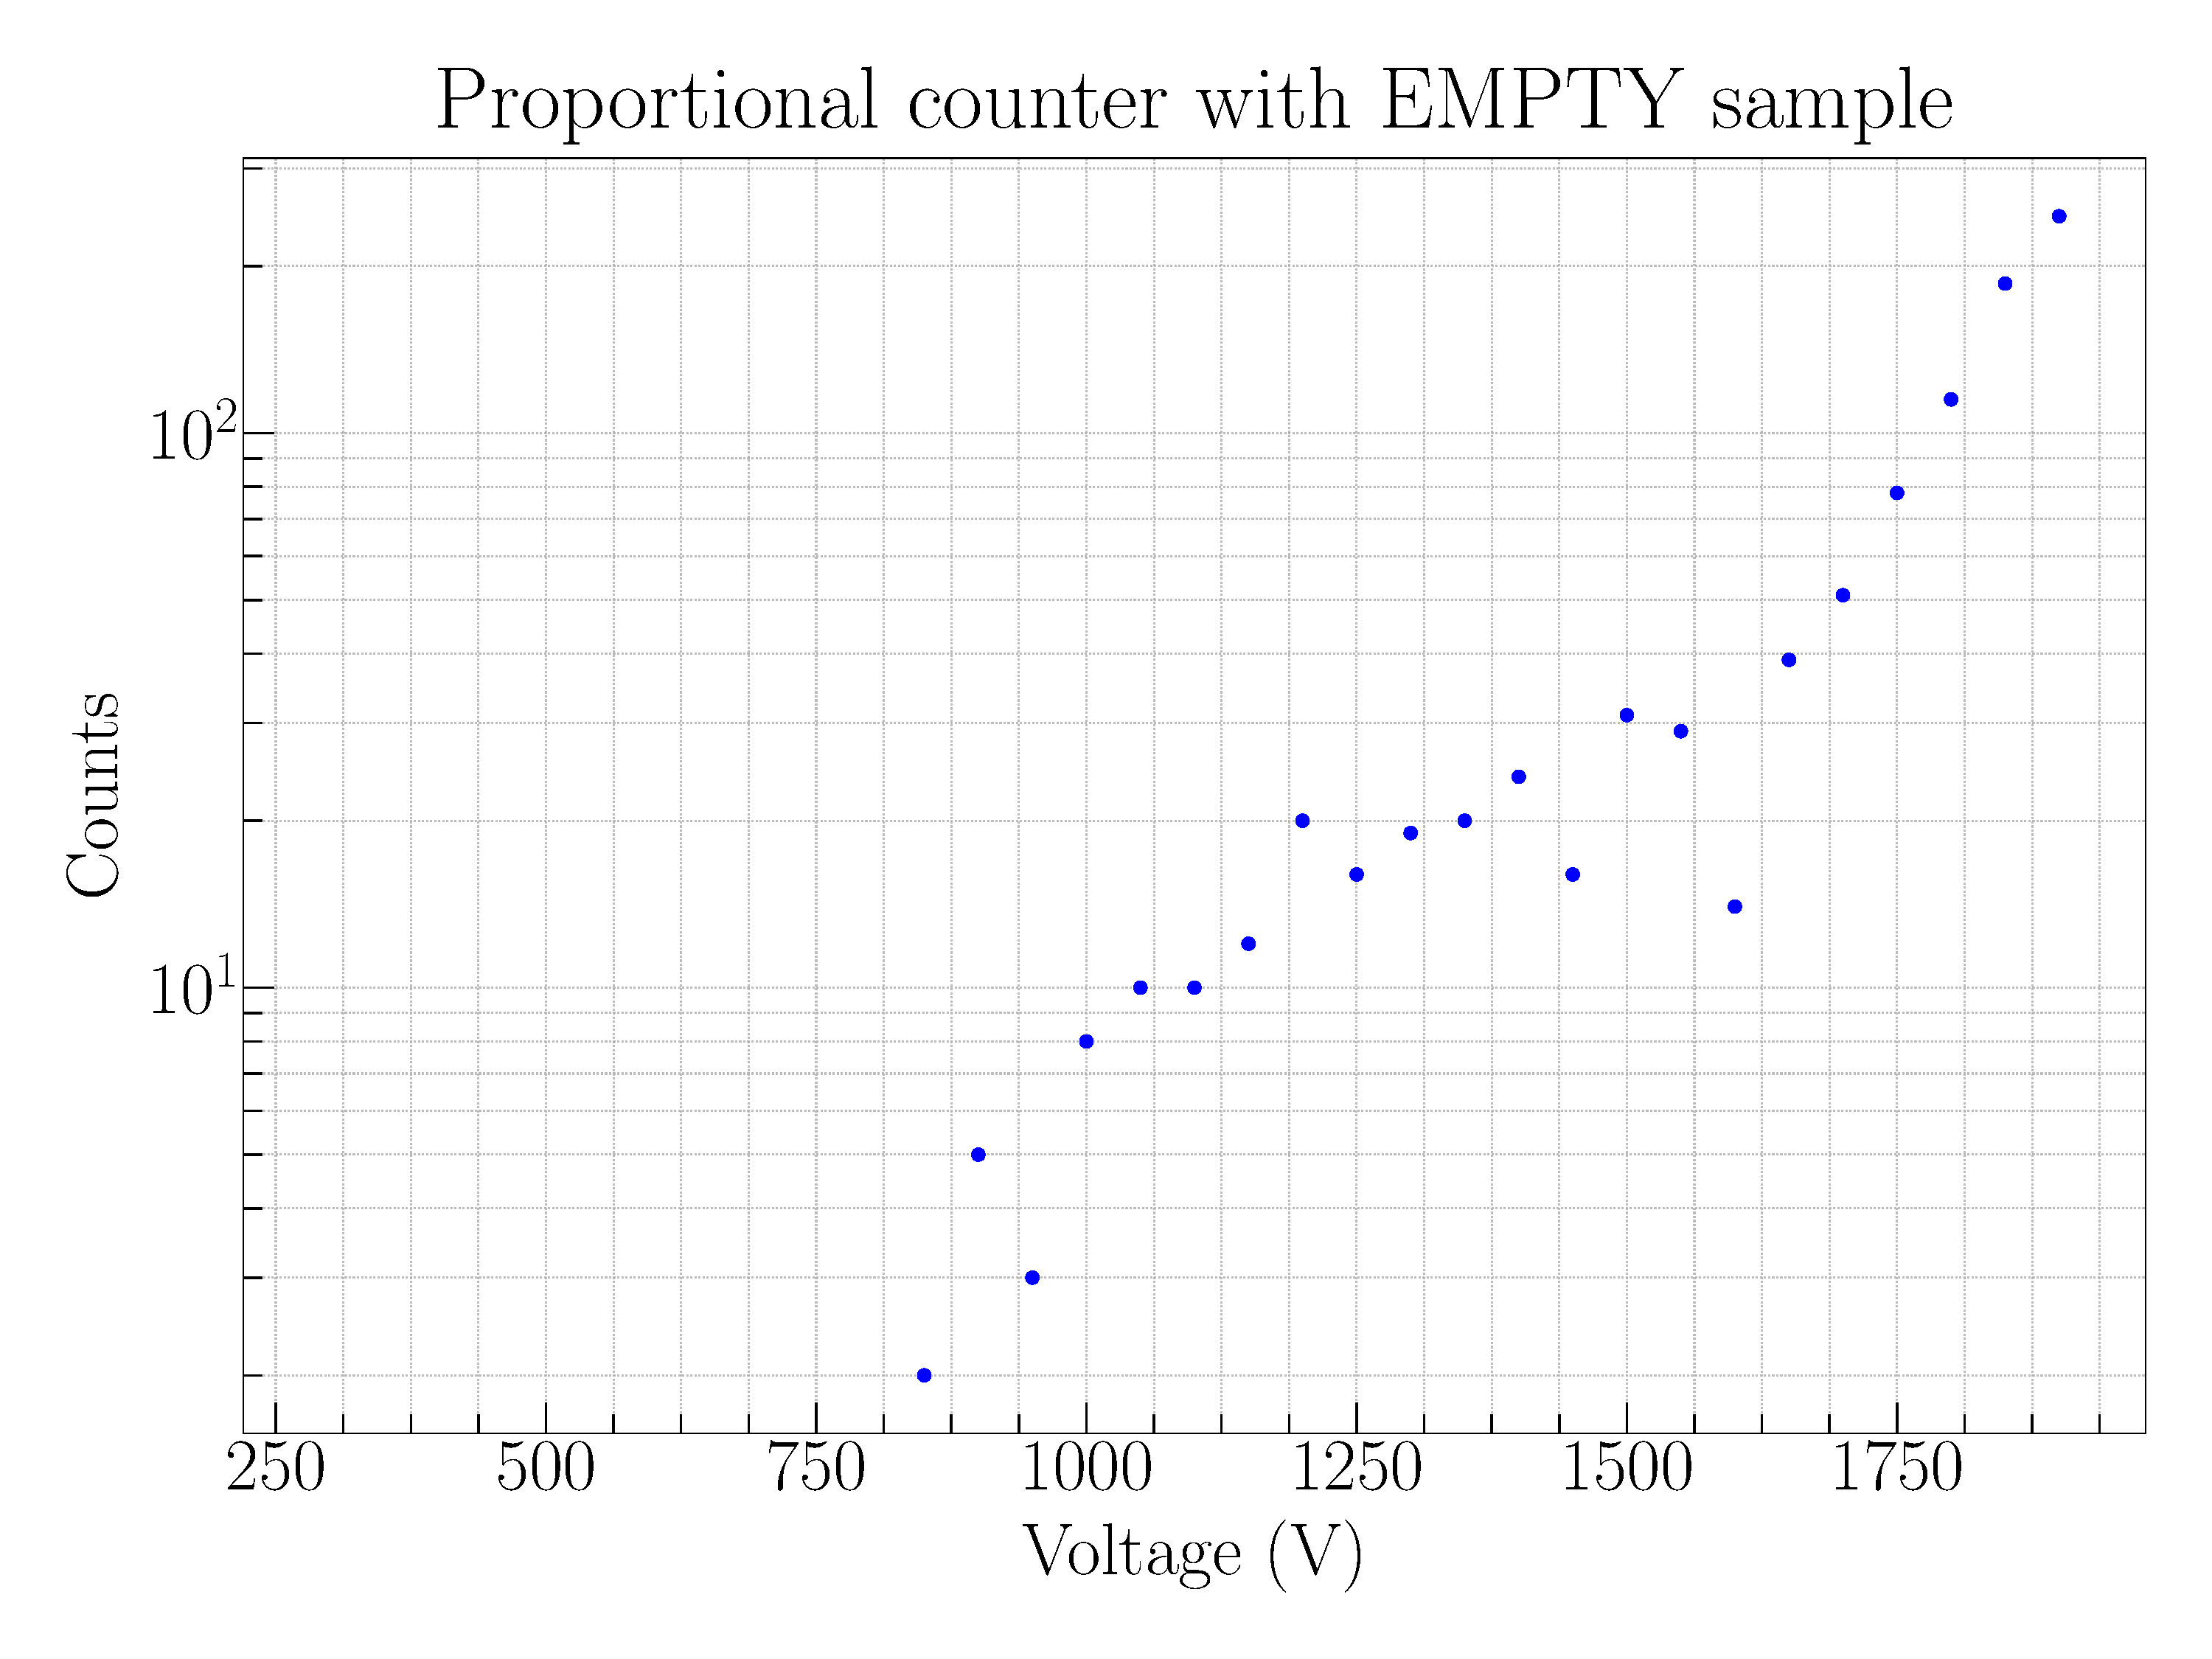
\includegraphics[width=0.8\textwidth]{../Figures/Proportional_characteristic_curve_EMPTY.pdf}
\caption{Characteristic curve of the empty detector.}
\label{fig:EmptyChar}
\end{figure}

\section{Conclusion}

The experiment went down with no complications. The analysed data shows that the characteristic curves of the counters behave as expected. When we look at the statistics, we see that the distributions we expected do show and the goodness tests seem to validate the hypothesis. One exception is the expected curve of the exponential distribution. The values we got were not comparable with the experimental data. It seems like some sort of scaling malfunction, but we were not able to find the cause for this. We also suspect that the $\chi^2$-test for the fitted exponential distribution can not be valid. Unfortunately we were not able to resolve these two issues even after consulting different sources and using different libraries for computation.

\end{document}
